\documentclass[12pt]{article}
\usepackage[pdfborder={0 0 0.5 [3 2]}]{hyperref}%
\usepackage[left=1in,right=1in,top=1in,bottom=1in]{geometry}%
\usepackage[shortalphabetic]{amsrefs}%
\usepackage{amsmath}
\usepackage{enumerate}
% \usepackage{enumitem}
\usepackage{amssymb}                
\usepackage{amsmath}                
\usepackage{amsfonts}
\usepackage{amsthm}
\usepackage{bbm}
\usepackage[table,xcdraw]{xcolor}
\usepackage{tikz}
\usepackage{float}
\usepackage{booktabs}
\usepackage{svg}
\usepackage{mathtools}
\usepackage{cool}
\usepackage{url}
\usepackage{graphicx,epsfig}
\usepackage{makecell}
\usepackage{array}

\def\noi{\noindent}
\def\T{{\mathbb T}}
\def\R{{\mathbb R}}
\def\N{{\mathbb N}}
\def\C{{\mathbb C}}
\def\Z{{\mathbb Z}}
\def\P{{\mathbb P}}
\def\E{{\mathbb E}}
\def\Q{\mathbb{Q}}
\def\ind{{\mathbb I}}

\DeclareMathOperator{\spn}{span}
\DeclareMathOperator{\ran}{range}

\graphicspath{ {periodic/} }

\newtheorem{lemma}{Lemma}
\newtheorem{theorem}{Theorem}
\newtheorem{corollary}{Corollary}
\newtheorem{definition}{Definition}
\newtheorem{assumption}{Assumption}
\newtheorem{proposition}{Proposition}
\newtheorem{hypothesis}{Hypothesis}

\newtheorem{notation}{Notation}

\begin{document}

\section{KdV5 with Periodic Boundary Conditions}

\subsection{Background}

In this section we will look at multipulse solutions to KdV5 in the case where we have periodic boundary conditions. Note that we cannot use an exponential weight in this case since our domain is of finite length. A periodic $n$-pulse is parameterized by the $n$ lengths $X_0, \dots, X_{n-1}$, where in general we will want one of the $X_i$ (representing the ``periodic piece'') to be larger than the others. (Since we have a periodic domain, for convenience we index the lengths starting with $X_0$ so that all the subscripts will be $\mod n$.) A diagram of a 2-pulse is shown below.

\begin{figure}[H]
\includegraphics[width=8.5cm]{dpimage}
\end{figure}

Let $X_m = \min \{ X_0, \dots, X_{n-1} \}$ and $X_M = \max \{ X_0, \dots, X_{n-1} \}$.\\

We would like to write the periodic multipulse as a small (piecewise) perturbation of the single pulse as was done in San98 (and San93). The method in those papers, however, does not give us the estimates we need for the stability problem. Instead, we will give another construction based on San97. This boils down to proving existence of the periodic multipulse, which is what we shall do. We assume that $c > 1/4$, since that is necessary for the existence of multipulses to KdV5. Thus the eigenvalues of the linearization about $0$ are complex and given by $\pm \alpha \pm \beta i$.\\

Since we are only interested in the existence problem here, we can use the 4th order (integrated) equation in the traveling frame

\begin{equation}\label{4thorder}
f(u) = u_{xxxx} - u_{xx} + c u - u^2 = 0
\end{equation}

This equation is Hamiltonian, with energy 

\begin{equation}\label{4thorderE}
H(u) = u_x u_{xxx} - \frac{1}{2}u_{xx}^2 - \frac{1}{2}u_x^2 + \frac{c}{2}u^2 - \frac{1}{3}u^3
\end{equation}

The Hamiltonian is conserved for any solution $u$ to \eqref{4thorder} since

\begin{align*}
\frac{d}{dx}H(u) = u_x(u_{xxxx} - u_{xx} + c u - u^2) = 0
\end{align*}

In what follows, we will write the problem as a first order system, i.e. we will take $U = (u_1, u_2, u_3, u_4) = (u, u_x, u_{xx}, u_{xxx})$. Then the problem becomes

\begin{equation}\label{4thordersystem}
U' = F(U) = \begin{pmatrix} 
u_2 \\ u_3 \\ u_4 \\ u_3 - c u_1 + u_1^2
\end{pmatrix}
\end{equation}

The Hamiltonian then takes the form

\begin{equation}
H(u_1, u_2, u_3, u_4) = u_2 u_4 - \frac{1}{2}u_3^2 - \frac{1}{2}u_2^2 + \frac{c}{2}u_1^2 - \frac{1}{3}u_1^3
\end{equation}

The gradient of the Hamiltonian is

\begin{equation}
\nabla H = (cu_1 - u_1^2, -u_2 + u_4, -u_3, u_2)
\end{equation}

It is straightforward to verify that $\langle F(U), \nabla H(U) \rangle = 0$ for all $U$.\\

The way we have written this, we can write our equation as $U' = \tilde{J} \nabla H$, where

\[
\tilde{J} = \begin{pmatrix}
0 & 0 & 0 & 1 \\
0 & 0 & -1 & 0 \\
0 & 1 & 0 & 1 \\
-1 & 0 & -1 & 0 \\
\end{pmatrix}
\]

This is not the standard symplectic matrix $J$, but $\tilde{J}$ is invertible and skew symmetric. \\

We note that 0 is an equilibrium of the system. Let $Q(x)$ be a homoclinic orbit connecting the equilibrium at 0 to itself. Such a homoclinic orbit is known to exist. Then since $Q(0)$ is not an equilibrium point of the system, we also know that $\nabla H(Q(0)) \neq 0$ since $\tilde{J}$ is invertible.

\subsection{Construction of Periodic Multipulses}

\subsubsection{Setup}

We look at the general equation

\begin{equation}\label{generaleq}
U'(x) = F(U)
\end{equation}

where $U \in \R^{2m}$ and $F$ is real-valued. (This should also extend to the complex-valued case.)\\

We take the following assumptions.

\begin{hypothesis}\label{assumptions}
\[\]
\begin{enumerate}
	\item $U = 0$ is a hyperbolic equilibrium of \eqref{generaleq}.
	\item There exists a homoclinic orbit $Q(x)$ connecting the equilibrium at 0 to itself.
	\item We have a nondegeneracy condition
	\[
	T_{Q(0)} W^u(0) \cap T_{Q(0)} W_s(0) = \R Q'(0)
	\]
	\item At least one of the following is true:
	\begin{enumerate}
		\item The system is reversible, and the homoclinic orbit $Q(x)$ is symmetric.
		\item The system is Hamiltonian, and $\nabla H(Q(0)) \neq 0$, where $H$ is the Hamiltonian energy
	\end{enumerate}
\end{enumerate}
\end{hypothesis}

By the nondegeneracy hypothesis, there exists a unique, bounded solution $\Psi(x)$ to the adjoint variational equation

\begin{equation}
W' = -D_U F(Q(x))^* W
\end{equation}

If we assume the system is Hamiltonian, we actually know the specific form of $\Psi(x)$.

% Lemma : Hamiltonian case

\begin{lemma}

If $U'(x) = F(U)$ is Hamiltonian, then

\begin{equation}
\Psi(x) = \nabla H(Q(x))
\end{equation}

where $H$ is the Hamiltonian energy associated with the system.

\begin{proof}

If the system is Hamiltonian, then $\langle F(Q(x)), \nabla H(Q(x)) \rangle = 0$ for all $x$. Taking the gradient of this and using known vector calculus identities, we have

\begin{align*}
0 &= \nabla \langle F(Q(x)), \nabla H(Q(x)) \rangle \\
&= D F(Q(x))^* \nabla H(Q(x)) + D^2 H(Q(x))^* F(Q(x)) \\
&= D F(Q(x))^* \nabla H(Q(x)) + D^2 H(Q(x)) Q'(x) \\
&= D F(Q(x))^* \nabla H(Q(x)) + \frac{d}{dx} \nabla H(Q(x))
\end{align*}

since the Hessian matrix is self-adjoint. Rearranging this, we have

\begin{equation}
\frac{d}{dx} \nabla H(Q(x)) = -D F(Q(x))^* \nabla H(Q(x)) 
\end{equation}

thus $\nabla H(Q(x))$ is a solution to the adjoint variational equation. Since $\nabla H$ is continuous and $Q(x)$ is bounded (even better, it decays exponentially to 0), so is $\nabla H(Q(x))$. By the nondegeneracy condition, there is a unique such solution, so we must have $\Psi(x) = \nabla H(Q(x))$.

\end{proof}
\end{lemma}

Next, we parameterize the stable and unstable manifolds near $Q(0)$. To do that we first write

\begin{align*}
T_{q(0)}W^u(0) &= \R Q'(0) \oplus Y^- \\
T_{q(0)}W^s(0) &= \R Q'(0) \oplus Y^+ \\
Z &= \R \Psi(0)
\end{align*}

By Hypothesis \ref{assumptions},

\[
\R^4 = \R Q'(0) \oplus Y^+ \oplus Y^- \oplus Z
\]
 
We have shown before that $Z$ is perpendicular to the other three. \\

We now write $W^u(0)$ and $W^s(0)$ as graphs over their own tangent spaces near $Q(0)$. Following San97, we can parameterize the unstable and stable manifolds near $Q(0)$ by the smooth functions

\begin{align*}
Q^-(\alpha, \beta^-) \\
Q^+(\alpha, \beta^+)
\end{align*}

where $\alpha \in \R$, $\beta^\pm \in Y^\pm$ and we have set things up so that $Q^+(\alpha, 0) - Q^-(\alpha, 0) \in Z$. Note that $Q^+(0, 0) = Q^-(0, 0) = Q(0)$. The parameter $\alpha$ is a phase parameter (which we will always take to be 0); although we could ignore it in our parameterization, we include it here to indicate that both manifolds are two-dimensional. \\

Next, we define the trajectories

\begin{align*}
Q^-(\alpha, \beta^-)(x) && x \leq 0 \\
Q^+(\alpha, \beta^-)(x) && x \geq 0
\end{align*}

which are the unique solutions to $U' = F(U)$ with ICs $Q^\pm(\alpha, \beta^\pm)$ for appropriate $x$. Note that since the ICs are on the stable/unstable manifolds, these decay exponentially in the appropriate direction with rate $\alpha$.\\

Using the parameterizations of the stable and unstable manifolds, we write the solution $U$ piecewise for $i = 0, \dots, n-1$ as

\begin{align*}
U_i^-(x) &= Q^-(0, \beta_i^-)(x) + V_i^-(x) && x \leq 0 \\
U_i^+(x) &= Q^+(0, \beta_i^+)(x) + V_i^+(x) && x \geq 0
\end{align*}

In essence, we are writing $U$ in terms of $2n$ parameters $\beta_i^\pm$ (representing ICs on the stable/unstable manifolds) and $n$ ``remainder'' functions $V_i^\pm(x)$.\\

We will choose $V_i^\pm(x)$ so that

\begin{align*}
V_i^-(0) &\in Z \oplus Y^- \\
V_i^+(0) &\in Z \oplus Y^+
\end{align*}

since the other directions are covered by $\beta_i^\pm$ (and $\alpha$, but we set that equal to 0).\\

Thus the problem we need to solve to construct the periodic multipulse is

\begin{align}
(U_i^\pm)' - F(U_i^\pm) &= 0 \\
U_i^+(X_i) - U_{i+1}^-(-X_i) &= 0 \\
U_i^+(0) - U_i^-(0) &= 0;
\end{align}

for $i = 0, \dots, {n-1}$. The subscripts are all mod $n$; in particular, $U_n^- = U_0^-$.\\

Let $\Phi_\pm(x, y; \beta^\pm)$ be the family of evolution operators for the variational equations

\begin{equation}
(V^\pm)' = D_U F(Q^\pm(0, \beta^\pm)(x)) V^\pm
\end{equation}

where these are defined on the appropriate interval. We can decompose these evolution operators via an exponential dichotomy.

\begin{lemma}\label{dichotomy1}
There exist projections

\begin{align*}
&P_+^s(y; \beta^+) && y \geq 0 \\
&P_+^u(y; \beta^+) = I - P_+^s(y; \beta^+) && y \geq 0 \\
&P_-^u(y; \beta^-) && y \leq 0 \\
&P_-^s(y; \beta^-) = I - P_-^u(y; \beta^-) && y \leq 0 \\
\end{align*}

such that the evolution operators $\Phi_\pm(x, y; \beta^\pm)$ can be decomposed as

\begin{align*}
\Phi^s_\pm(x, y; \beta^\pm) &= \Phi_\pm(x, y; \beta^\pm) P^s_\pm(y; \beta^\pm) \\
\Phi^u_\pm(x, y; \beta^\pm) &= \Phi_\pm(x, y; \beta^\pm) P^u_\pm(y; \beta^\pm) 
\end{align*}

where we have the estimates

\begin{align*}
|\Phi^s_+(x, y, \beta^+)| &\leq C e^{-\alpha(x - y)} && 0 \leq y \leq x \\
|\Phi^u_+(x, y, \beta^+)| &\leq C e^{-\alpha(y - x)} && 0 \leq x \leq y \\
|\Phi^u_-(x, y, \beta^+)| &\leq C e^{-\alpha(y - x)} && 0 \geq y \geq x \\
|\Phi^s_-(x, y, \beta^+)| &\leq C e^{-\alpha(x - y)} && 0 \geq x \geq y \\
\end{align*}

which also hold for derivatives with respect to the ICs $\beta^\pm$. In addition, the projections satisfy 

\begin{align*}
\Phi_\pm(x, y; \beta^\pm) P^{s/u}_\pm(y; \beta^\pm) 
= P^{s/u}_\pm(x; \beta^\pm) \Phi_\pm(x, y; \beta^\pm)
\end{align*}

i.e. it does not matter if we project or evolve first. Finally, the projections can be chosen such that at $y = 0$ we have, independent of $\beta^+$ and $\beta^-$

\begin{align*}
\ker P^s_+(0; \beta^+) &= Z \oplus Y^- \\
\ker P^u_-(0; \beta^-) &= Z \oplus Y^+ \\
\ran P^u_+(0; \beta^+) &= Z \oplus Y^- \\
\ran P^s_-(0; \beta^-) &= Z \oplus Y^+
\end{align*}

\begin{proof}
Since $D_U F(0)$ is hyperbolic by assumption, this follows from Lemma 5.1 in San97, which follows from Lemma 1.1 in San93.
\end{proof}
\end{lemma}

The next lemma is a bound on the difference between the exponential dichotomy projections and the projections onto the stable and unstable eigenspaces.

% lemma : bound on projection difference

\begin{lemma}\label{p1}

Let 

\begin{equation}
p_1(X; \beta^+, \beta^-) = \sup_{x \geq X} (|P^u_+(x; \beta^+) - P_0^u| + |P^s_-(-x; \beta^-) - P_0^s|)
\end{equation}

Then we have the $X$-dependent bound

\begin{equation}
p_1(X; \beta^+, \beta^-) = \mathcal{O}(e^{-\alpha X})
\end{equation} 

\begin{proof}
This follows from Lemma 1.1 in San93.
\end{proof}

\end{lemma}

% rewrite piecewise

Next, we rewrite the problem $U'(x) = F(U)$ in piecewise fashion in such a way as to exploit what we did above. We want to solve piecewise

\begin{align*}
(U_i^\pm(x))' &= (Q^\pm(0, \beta_i^\pm)(x))' + (V_i^\pm(x))' = F\left(Q^\pm(0, \beta_i^\pm)(x) + V_i^\pm(x) \right) \\
\end{align*}

for $i = 0, \dots, n-1$. Using the fact that (by construction) $Q^\pm(0, \beta_i^\pm)(x)$ solves $U'(x) = F(U)$ on the appropriate interval, this becomes

\begin{align*}
F(Q^\pm(0, \beta_i^\pm)(x)) + (V_i^\pm(x))' &= F(Q^\pm(0, \beta_i^\pm)(x) + V_i^\pm(x) )
\end{align*}

Solving for $(V_i^\pm(x))'$, we have

\begin{align*}
(V_i^\pm(x))' &= F(Q^\pm(0, \beta_i^\pm)(x) + V_i^\pm(x) ) - F(Q^\pm(0, \beta_i^\pm)(x) )
\end{align*}

Now we Taylor about $F(Q^\pm(0, \beta_i^\pm)(x)$ to get the equivalent formulation

\begin{equation}\label{Vpiecewise}
(V_i^\pm(x))' = D_U F(Q^\pm(0, \beta_i^\pm)(x)) V_i^\pm(x)  + G_i^\pm(\beta_i^\pm, V_i^\pm)(x)
\end{equation}

where 

\begin{equation}\label{Gquadratic}
G_i^\pm(\beta_i^\pm, V_i^\pm)(x) = \mathcal{O}(|V_i^\pm|^2)
\end{equation}

independent of the parameters $\beta_i^\pm$. The fact that this is bound is independent of the $\beta_i^\pm$ follows from the fact that we have bounds on $Q^\pm(0, \beta_i^\pm)$ which are independent of $\beta_i^\pm$. Derivatives of $G_i^\pm$ with respect to the parameters $\beta_i^\pm$ are the same order in $V_i^\pm$.\\

At this point, we rewrite the (piecewise) differential equations \eqref{Vpiecewise} in integrated form as fixed point equations. Recall again that the subscripts are mod $n$, so that, for example, $X_0 = X_n$. Thus we have

\begin{align*}
V_i^+(x) &= \Phi^u_+(x, X_i; \beta_i^+) a_i^+  \\
&+ \int_{X_i}^x \Phi_+^u(x, y; \beta_i^+) G_i^+(y, V_i^+(y),\beta_i^+)dy \\
&+ \int_0^x \Phi_+^s(x, y, \beta_i^+) G_i^+(y, V_i^+(y),\beta_i^+)dy \\ 
V_i^-(x) &= \Phi^s_-(x, -X_{i-1}, \beta_i^-) a_{i-1}^-  \\
&+ \int_{-X_{i-1}}^x \Phi_-^s(x, y, \beta_i^-) G_i^-(y, V_i^-(y),\beta_i^-)dy \\
&+ \int_0^x \Phi_-^u(x, y, \beta_i^-) G_i^-(y, V_i^-(y),\beta_i^-)dy \\
\end{align*}

where for the initial conditions $a_i^\pm$ we have

\begin{align*}
a_i^+ &\in E_0^u \\
a_i^- &\in E_0^s \\
\end{align*}

Note that we do not have initial conditions $b_i^\pm$ at $x = 0$ for the other side of the dichotomy. Since these ICs would live in $Y^\pm$, we have incorporated them into the $\beta_i^\pm$.\\

Next, we define the exponentially weighted norms

\begin{align*}
||V||_{X, +} = \sup_{x \in [0, X]} e^{\alpha(X - x)}|V(x)| \\
||V||_{X, -} = \sup_{x \in [-X, 0]} e^{\alpha(X + x)}|V(x)| \\
\end{align*}

Let $K_{X, +}$ be the spaces on continuous functions on the appropriate intervals equipped with these norms. These are known to be Banach spaces. Let $B_{X, \pm}(\rho)$ be the ball of radius $\rho$ in these spaces.\\

\subsubsection{Inversion}

We will solve for the $V_i^\pm$ and the $\beta_i^\pm$ in a series of lemmas.\\

First, we solve for the functions $V_i^\pm(x)$ in terms of the initial conditions $a_i^\pm$. Note that $V_i^+(x)$ only depends on $a_i^+$ and $V_i^-(x)$ only depends on $a_{i-1}^-$

% lemma : solve for V_i^\pm

\begin{lemma}
There exist $\delta, \rho > 0$ such that for $|X_i| > 1/\delta$ and $|\beta_i^\pm| < \delta$, there exist unique solutions

\begin{align*}
V_i^-(a_{i-1}, \beta_i^-) &\in B_{X_{i-1}, -}(\rho) \\
V_i^+(a_i, \beta_i^+) &\in B_{X_i, +}(\rho) \\
\end{align*}

These depend smoothly on the $\beta_i^\pm$, and we have the estimates

\begin{align*}
||V_i^-||_{X_{i-1}, -} &\leq C |a_{i-1}^-| \\
||V_i^+||_{X_i, +} &\leq C |a_i^+|
\end{align*}

The estimates hold as well for derivatives of $V_i^\pm$ with respect to $\beta_i^\pm$.

\begin{proof}
This should just be Lemma 5.2 in San97. The following is a mostly filled-in version of that proof.\\

We can deal with the $2n$ pieces separately, so let's do the ``positive'' pieces here. The RHS of the fixed point equations defines a smooth mapping on $K_{X_i, +}$ (basically obvious since everything involved is smooth, although we could check this). We need to verify that the RHS maps to $K_{X_i, +}$, so we check the three terms individually. We use our estimates on $\Phi^{s/u}_\pm$ from Lemma \ref{dichotomy1} and $G$ from \ref{Gquadratic} and the fact that $V_i^+ \in K_{X_i, +}$.\\

For the first term, we have

\begin{align*}
e^{\alpha(X_i - x)} | \Phi^u_+(x, X_i; \beta_i^+) a_i^+ | 
&\leq C e^{\alpha(X_i - {}x} e^{-\alpha(X_i - x)} |a_i^+| \\
&\leq C |a_i^+|
\end{align*}

For the second term,

\begin{align*}
e^{\alpha(X_i - x)} &\left| \int_{X_i}^x \Phi_+^u(x, y; \beta_i^+) G_i^+(y, V_i^+(y),\beta_i^+)dy  \right| \\
&\leq C e^{\alpha(X_i - x)} \int_x^{X_i} e^{-\alpha(y - x)}|V_i^+(y)|^2 dy \\
&\leq C e^{\alpha(X_i - x)} \int_x^{X_i} 
e^{-\alpha(y - x)}(e^{-\alpha(X_i - y)})^2|e^{\alpha(X_i - y)} V_i^+(y)|^2 dy \\
&\leq C e^{\alpha(X_i - x)} \int_x^{X_i} 
e^{-\alpha(y - x)}(e^{-\alpha(X_i - y)})^2 dy \\
&\leq C \int_0^{X_i} e^{-\alpha (X_i - y)} dy \\
&\leq C
\end{align*}

The third term is similar. Thus the RHS of the fixed point equations does indeed map $K_{X_i, +}$ to itself.\\

Now that we know what spaces things live in, define 
$H: K_{X_i, +} \times E_0^s \rightarrow K_{X_i, +}$ by

\begin{align*}
H(V_i^+(x), a_i^+, \beta_i^+) &= V_i^+(x) - \Phi^u_+(x, X_i; \beta_i^+) a_i^+  \\
&- \int_{X_i}^x \Phi_+^u(x, y; \beta_i^+) G_i^+(y, V_i^+(y),\beta_i^+)dy \\
&- \int_0^x \Phi_+^s(x, y; \beta_i^+) G_i^+(y, V_i^+(y),\beta_i^+)dy 
\end{align*}

Since $Q(x)$ satisfies the original ODE, we know that $H(0, 0, 0) = 0$. We can check that the Frechet derivative of $H$ with respect to $V_i^+$ at $(V_i^+(x), a_i^+, \beta_i^+) = (0, 0, 0)$ is a Banach space isomorphism on $K_{X_i, +}$. Then using the implicit function theorem, we can solve for $V_i^+(x)$ in terms of $(a_i^+, \beta_i^+)$. This dependence is smooth, since the map $H$ is smooth. $V_i^-(x)$ is similar. \\

The estimate on $V_i^\pm$ comes from the estimate of the first term on the RHS of the fixed point equations, since the other terms (those involving the integrals) are quadratic in $V_i^\pm$. 

\end{proof}
\end{lemma}

Next, we look at the conditions $U_i^+(X_i) - U_{i+1}^-(-X_i) = 0$.

% Lemma : solve for a_i^\pm

\begin{lemma}\label{solvefora}
For any $X_i$ and $\beta_i^\pm$ chosen as in the previous lemma, there is a unique pair of initial conditions $(a_i^+, a_i^-) \in E_0^s \times E_0^u$ such that $U_i^+(X_i) - U_{i+1}^-(-X_i) = 0$. $(a_i^+, a_i^-)$ depends smoothly on $(\beta_i^+, \beta_{i+1}^-)$, and we have the following estimate, which is independent of $(\beta_i^+, \beta_{i+1}^-)$.

\begin{equation}
|a_i^\pm| \leq C e^{-\alpha X_i}
\end{equation}

which holds for $a_i^\pm$ as well as derivatives with respect to $\beta_i^\pm$.\\

We also have the following expressions for the $a_i^\pm$

\begin{align*}
a_i^+ &= P^s_0 \left( Q^+(0, \beta_i^+)(X_i) - Q^-(0, \beta_{i+1}^-)(-X_i) \right) 
+ \mathcal{O}( e^{-2 \alpha X_i} )\\
a_i^- &= P^u_0 \left( Q^+(0, \beta_i^+)(X_i) - Q^-(0, \beta_{i+1}^-)(-X_i) \right) 
+ \mathcal{O}( e^{-2 \alpha X_i} )
\end{align*}

\begin{proof}

First, plug in the fixed point equations to the expressions for $U_i^+$ and $U_{i+1}^-$ and evaluate them at $\pm X_i$ to get
\begin{align*}
U_i^+(X_i) &= Q^+(0, \beta_i^+)(X_i) + P^u_+(X_i; \beta_i^+) a_i^+ \\
&+ \int_0^{X_i} \Phi_+^s(X_i, y; \beta_i^+) G_i^+(y, V_i^+(y),\beta_i^+)dy \\ 
U_{i+1}^-(-X_i) &= Q^-(0, \beta_{i+1}^-)(-X_i) + P^s_-(-X_i; \beta_{i+1}^-) a_i^- \\
&+ \int_0^{-X_i} \Phi_-^u(-X_i, y; \beta_{i+1}^-) G_{i+1}^-(y, V_{i+1}^-(y),\beta_{i+1}^-)dy \\
\end{align*}

Adding and subtracting $P_0^{s/u}$ and recalling where the $a_i^\pm$ live, this becomes

\begin{align*}
U_i^+(X_i) &= Q^+(0, \beta_i^+)(X_i) + a_i^+ + (P^u_+(X_i; \beta_i^+) -  P^u_0)a_i^+ \\
&+ \int_0^{X_i} \Phi_+^s(X_i, y; \beta_i^+) G_i^+(y, V_i^+(y),\beta_i^+)dy \\ 
U_{i+1}^-(-X_i) &= Q^-(0, \beta_{i+1}^-)(-X_i) + a_i^- + (P^s_-(-X_i; \beta_{i+1}^-) - P^s_0) a_i^- \\ 
&+ \int_0^{-X_i} \Phi_-^u(-X_i, y; \beta_{i+1}^-) G_{i+1}^-(y, V_{i+1}^-(y),\beta_{i+1}^-)dy \\
\end{align*}

Subtracting these, we obtain the equation we need to solve

\begin{align*}
0 &= H(a_i^+, a_i^-, \beta_i^+, \beta_{i+1}^-) \\
&= a_i^+ - a_i^- + (P^u_+(X_i; \beta_i^+) -  P^u_0)a_i^+ - (P^s_-(-X_i; \beta_{i+1}^-) - P^s_0) a_i^-  \\
&+ Q^+(0, \beta_i^+)(X_i) - Q^-(0, \beta_{i+1}^-)(-X_i)\\
&+ \int_0^{X_i} \Phi_+^s(X_i, y; \beta_i^+) G_i^+(y, V_i^+(y),\beta_i^+)dy
- \int_0^{-X_i} \Phi_-^u(-X_i, y; \beta_{i+1}^-) G_{i+1}^-(y, V_{i+1}^-(y),\beta_{i+1}^-)dy 
\end{align*}

where $H: E_0^s \times E_0^u \times \R \times \R \rightarrow \R^4$. In the previous lemma, we solved for $V_i^\pm$ in terms of the $a_i^\pm$ and $\beta_i^\pm$, so we plug that in to get

\begin{align*}
H(a_i^+, &a_i^-, \beta_i^+, \beta_{i+1}^-) \\
&= a_i^+ - a_i^- + (P^u_+(X_i; \beta_i^+) -  P^u_0)a_i^+ - (P^s_-(-X_i; \beta_{i+1}^-) - P^s_0) a_i^-  \\
&+ Q^+(0, \beta_i^+)(X_i) - Q^-(0, \beta_{i+1}^-)(-X_i)\\
&+ \int_0^{X_i} \Phi_+^s(X_i, y; \beta_i^+) G_i^+(y, V_i^+(a_i^+, \beta_i^+)(y),\beta_i^+)dy \\
&- \int_0^{-X_i} \Phi_-^u(-X_i, y; \beta_{i+1}^-) G_{i+1}^-(y, V_{i+1}^-(a_i^-, \beta_{i+1}^-)(y),\beta_{i+1}^-)dy 
\end{align*}

Again, note that $H(0, 0, 0, 0) = 0$. We want to solve for $a_i^\pm$ using the implicit function theorem, so we need to look at $D_{a_i^\pm} H(0, 0, 0, 0)$.\\

When we differentiate with respect to $a_i^\pm$ at $a_i^\pm = 0$, we note that the the derivatives of the integral terms in $H$ will be 0 since $G_i^\pm$ is quadratic order in $V_i^\pm$, thus quadratic order in $a_i^\pm$ by the previous lemma. The $Q^\pm$ terms do not involve $a_i^\pm$.\\

Thus, taking the partial derivative with respect to $a_i^\pm = 0$, we get

\[
\frac{\partial}{\partial a_i^\pm} H(0, 0, 0, 0) = \pm 1 + \mathcal{O} (e^{-\alpha X_i})
\]

Thus, for sufficiently large $X_i$, $D_{a_i^\pm} H(0, 0, 0, 0)$ is invertible in a neighborhood of $(0, 0, 0, 0)$, so we can use the IFT to solve for $a_i^\pm$ in terms of $\beta_i^\pm$. \\

Now that we have found $a_i^\pm$ which satisfies the $H(a_i^+, a_i^-, \beta_i^+, \beta_{i+1}^-) = 0$, we can get an expression and estimates for the $a_i^\pm$. Recalling the spaces $a_i^\pm$ live in, we apply the projection $P^s_0$ to get

\begin{align*}
0 &= a_i^+ + P^s_0(P^u_+(X_i; \beta_i^+) -  P^u_0)a_i^+ 
+ P^s_0 \left( Q^+(0, \beta_i^+)(X_i) - Q^-(0, \beta_{i+1}^-)(-X_i) \right)\\
&+ P^s_0 \left( \int_0^{X_i} \Phi_+^s(X_i, y; \beta_i^+) G_i^+(y, V_i^+(a_i^+, \beta_i^+)(y),\beta_i^+)dy \right) \\
&- P^s_0 \left( \int_0^{-X_i} \Phi_-^u(-X_i, y; \beta_{i+1}^-) G_{i+1}^-(y, V_{i+1}^-(a_i^-, \beta_{i+1}^-)(y),\beta_{i+1}^-) dy \right)
\end{align*}

We have estimates for all of these terms. For the first two terms, we have

\begin{align*}
|P^s_0(P^u_+(X_i; \beta_i^+) -  P^u_0)a_i^+ | &\leq C e^{-\alpha X_i} |a_i^+| \\
|P^s_0 \left( Q^+(0, \beta_i^+)(X_i) - Q^-(0, \beta_{i+1}^-)(-X_i) \right)| &\leq C e^{-\alpha X_i}.
\end{align*}

using Lemma \ref{p1}. For the integral terms, we have

\begin{align*}
\left| \int_0^{X_i} \Phi_+^s(X_i, y; \beta_i^+) G_i^+(y, V_i^+(a_i^+, \beta_i^+)(y),\beta_i^+)dy \right| &\leq C \int_0^{X_i}e^{-\alpha(X_i - y)} |V_i^+(y)|^2 dy \\
&\leq C \int_0^{X_i}e^{-3 \alpha (X_i - y)} |e^{\alpha(X_i - y)} V_i^+(y)|^2 dy \\
&\leq C \int_0^{X_i}e^{-3 \alpha (X_i - y)} (||V_i^+||_{X_i, +})^2 dy \\
&\leq C |a_i^+|^2
\end{align*}

The other integral term is similar. In a hand-wavey fashion, we have something which looks like

\[
|a_i^+|(1 + \mathcal{O}(e^{-\alpha X_i}) + \mathcal{O}(|a_i^+|)) = 
\mathcal{O}( e^{-\alpha X_i} )
\]

which should give us the estimate we want

\begin{align*}
|a_i^\pm| \leq C e^{-\alpha X_i}
\end{align*}

To get an actual expression for $a_i^\pm$, we plug in all our estimates to get

\begin{align*}
a_i^+ = P^s_0 \left( Q^+(0, \beta_i^+)(X_i) - Q^-(0, \beta_{i+1}^-)(-X_i) \right) 
+ \mathcal{O}( e^{-2 \alpha X_i} )
\end{align*}

Similarly, we have

\begin{align*}
a_i^- = P^u_0 \left( Q^+(0, \beta_i^+)(X_i) - Q^-(0, \beta_{i+1}^-)(-X_i) \right) 
+ \mathcal{O}( e^{-2 \alpha X_i} )
\end{align*}

\end{proof}
\end{lemma}

Finally, we need the pieces to match at $x = 0$. In other words, we need to find $\beta_i^\pm$ such that $U_i^+(0) = U_i^-(0)$, i.e. 

\begin{align*}
Q^+(0, \beta_i^+) + V_i^+(0) &= Q^-(0, \beta_i^-) + V_i^-(0) && i = 0, \dots, n-1
\end{align*}

Before we do that, we will need to make a smooth change of coordinates near $Q(0)$. We will do that using a variation of the ``flow-box'' method. What we want to do is straighten out the stable and unstable manifolds near $Q(0)$ so that their non-intersecting directions lie along $Y^+$ and $Y^-$.

% lemma : straighten out manifolds

\begin{lemma}\label{straightenW}

There exists a differentiable map 

\[
H: \R \times Y^- \times Y^+ \times Z \rightarrow \R^4
\]

such that $H(0, 0, 0, 0) = Q(0)$, $H$ is invertible in a neighborhood of $Q(0)$, and

\begin{align*}
H^{-1}(Q^-(0, \beta^-) &= \beta^- \in Y^- \\
H^{-1}(Q^+(0, \beta^+) &= \beta^+ \in Y^+ \\
\end{align*}

for sufficiently small $\beta^\pm$.

\begin{proof}
We know that $Q'(0) = F(Q(0)) \neq 0$, i.e. the center of the pulse is not an equilibrium of the vector field $F$. Recall that $\R^4 = Z \oplus \R Q'(0) \oplus Y^+ \oplus Y^-$.\\

Let $S_y(P)$ be the solution operator for the ODE $U' = F(U)$, i.e. the operator which takes an initial condition $P$ and maps it to the point $H(y)$, where $H$ is the unique solution to $U' = F(U)$ such that $H(0) = P$.\\

Define the map $H: \R \times Y^- \times Y^+ \times Z \rightarrow \R^4$ by 

\begin{equation}
H(y; \beta^-, \beta^+, \gamma) = S_y(Q(0) + Q^-(0, \beta^-) + Q^-(0, \beta^+) + \gamma \Psi(0))
\end{equation}

In other words, $H(y; \beta^-, \beta^+, \gamma)$ is a trajectory of $U' = F(U)$ with initial condition $Q(0) + Q^-(\beta^-,0) + Q^-(\beta^+,0) + \gamma \Psi(0)$.\\ 

Near $Q(0)$, i.e. for small $x, \beta^\pm$ the stable and unstable manifolds are given by the curves

\begin{align*}
W^u &= H(x; \beta^-, 0, 0) \\
W^s &= H(x; 0, \beta^+, 0) 
\end{align*}

Their one-dimensional intersection is the homoclinic orbit $Q(x) = H(x; 0, 0, 0)$, whose tangent space is $Q'(x)$.\\

To complete the proof, we need to show that $H$ is invertible in a neighborhood of the origin. To compute the Jacobian of $H$ at the origin, we note the following.

\begin{align*}
H_y(0, 0, 0, 0) &= F(Q(0)) = Q'(0) \\
H_{\beta^-}(0, 0, 0, 0) &= (Q^-)_{\beta^-}(0,0) = Y^- \\
H_{\beta^+}(0, 0, 0, 0) &= (Q^+)_{\beta^+}(0,0) = Y^+ \\
H_{\gamma}(0, 0, 0, 0) &= Z
\end{align*}

Since $\R^4 = Z \oplus \R Q'(0) \oplus Y^+ \oplus Y^-$, the four partial derivatives of $H$ at the origin are linearly independent, thus the Jacobian of $H$ at the origin is invertible. Note that $H_y(0, 0, 0, 0) = Q(0)$. By the inverse function theorem, there exists open neighborhoods $N_1$ of 0 and $N_2$ of $Q(0)$ such that $H(N_1) = N_2$ and $H$ is invertible on $N_2$. \\

In particular, we have for sufficiently small $\beta^\pm$

\begin{align*}
H^{-1}(Q^-(0, \beta^-) &= \beta^- \in Y^- \\
H^{-1}(Q^+(0, \beta^+) &= \beta^+ \in Y^+ \\
\end{align*}

\end{proof}
\end{lemma}

Now we are ready to perform the match at $x = 0$ to solve for $\beta_i^\pm$. Before we do that, we change coordinates according to the prior lemma. In the new coordinates, near $Q(0)$ our ODE becomes

\begin{equation}
\tilde{U}' = DH(H^{-1}(\tilde{U})) F( H^{-1}(\tilde{U}) )
\end{equation}

where $H$ is defined in the previous lemma. If we match the $\tilde{U}_i^\pm$ at $x = 0$, then since $H^{-1}$ is a homeomorphism near $Q(0)$, we have also matched the $U_i^\pm$ at $x = 0$. For convenience, we will continue to write the ODE as $U' = F(U)$ after the coordinate change.\\

Note that because of our coordinate change, we have

\begin{align*}
P_Z(Q^\pm(0, \beta^\pm) &= 0 \\
P_{\R Q'(0)}(Q^\pm(0, \beta^\pm) &= 0 \\
P_{Y^\pm}(Q^\pm(\beta^\pm, 0)) &= \beta^\pm
\end{align*}

We wish to solve $U_i^+(0) - U_i^-(0) = 0$. Since $\R^4 = Z \oplus \R Q'(0) \oplus Y^+ \oplus Y^-$, it suffices to project this onto these four subspaces and solve separately on each subspace. Since $V_i^\pm(0) \in Z \oplus Y^\pm$, the projection on $\R Q'(0)$ is automatically 0. Thus we only need to solve the equations

\begin{align*}
P_{Y^\pm}(U_i^+(0) - U_i^-(0)) &= 0 \\
P_Z(U_i^+(0) - U_i^-(0)) &= 0 \\
\end{align*}

We will do each of these in turn. In the next lemma, we solve for $(\beta_i^+, \beta_i^-)$ for $i = 0, \dots, n-1$. We do this for each pair separately.

% lemma : solve for the \beta_i^\pm

\begin{lemma}\label{solveforbeta}
For $i = 0, \dots, n-1$ ,there exist $(\beta_i^+, \beta_i^-)$ such that $P_{Y^\pm}(U_i^+(0) - U_i^-(0)) = 0$ . We have the estimate

\begin{equation}
| (\beta_i^+, \beta_i^-) | \leq C (e^{-2 \alpha X_i} + e^{-2 \alpha X_{i-1}})
\end{equation}

\begin{proof}
Recall that $U_i^\pm = Q^\pm(0, \beta_i^\pm) + V_i^\pm$. Then since we have applied the change of coordinates above, we have

\begin{align*}
P_{Y^\pm}(Q^+(0, \beta_i^+) - Q^-(0, \beta_i^-)) &= \beta_i^+ - \beta_i^-
\end{align*}

Then the equation we want to solve becomes

\begin{equation}
H(\beta_i^+, \beta_i^-) = \beta_i^+ - \beta_i^- 
+ P_{Y^\pm}(V_i^+(0) - V_i^-(0)) = 0
\end{equation}

Substituting the fixed point equations evaluated at $x = 0$, we get

\begin{align*}
H(\beta_i^+, \beta_i^-) &= \beta_i^+ - \beta_i^- \\
&+ P_{Y^\pm} \Big( \Phi^u_+(0, X_i; \beta_i^+) a_i^+ 
+ \int_{X_i}^0 \Phi_+^u(0, y; \beta_i^+) G_i^+(y, V_i^+(y),\beta_i^+)dy \\
&- \Phi^s_-(0, -X_{i-1}, \beta_i^-) a_{i-1}^- 
- \int_{-X_{i-1}}^0 \Phi_-^s(0, y, \beta_i^-) G_i^-(y, V_i^-(y),\beta_i^-) dy \Big) 
\end{align*}

Next, since $\text{Ran }P_+^u(0; \beta^+) = Z \oplus Y^-$, the terms involving $\Phi^u_+$ can have no component in $Y^+$. Similarly, since $\text{Ran }P_-^s(0; \beta^-) = Z \oplus Y^+$, the terms involving $\Phi^s_-$ can have no component in $Y^-$. Thus we can separate our equation into the individual projections on $Y^-$ and $Y^+$. Redefining $H$ this way gives us

\begin{equation}
H(\beta^+, \beta^-) = 
\begin{pmatrix}
\beta_i^+ - P_{Y^+}\left(\Phi^s_-(0, -X_{i-1}, \beta_i^-) a_{i-1}^- 
- \int_{-X_{i-1}}^0 \Phi_-^s(0, y, \beta_i^-) G_i^-(y, V_i^-(y),\beta_i^-) dy\right) \\
\beta_i^- - P_{Y^-}\left( \Phi^u_+(0, X_i; \beta_i^+) a_i^+ 
+ \int_{X_i}^0 \Phi_+^u(0, y; \beta_i^+) G_i^+(y, V_i^+(y),\beta_i^+)dy \right)
\end{pmatrix}
\end{equation}

Note the the $\beta_i^\pm$ ``mix''. What we would like to do now is invert this to solve for the $\beta_i^\pm$. This requires estimating the partial derivatives with respect to $\beta_i^\pm$ of the two terms. Since the estimates for $G$ and $\Phi$ also apply to the derivatives with respect to $\beta_i^\pm$, this is not hard to do.\\

For the $a_i^\pm$ terms we have

\begin{align*}
\left| \frac{\partial}{\partial \beta_i^+} \Phi^u_+(\beta_i^+, 0, X_i) a_i^+ \right| \leq C e^{-\alpha X_i}|a_i^+|
& \leq C e^{-2 \alpha X_i}
\end{align*}

where we used our estimate for $a_i^\pm$ from above. The $\beta_i^-$ term is similar, except it involves $X_{i-1}$. For the integral terms, we have

\begin{align*}
\left| \frac{\partial}{\partial \beta_i^-} \int_{-X_{i-1}}^0 \Phi_-^s(\beta_i^-, 0, y) G^-(y, V^-(y),\beta^-)dy \right| 
&\leq C \int_{-X_{i-1}}^0 e^{\alpha y} | V_i^-(y) |^2 dy \\
&\leq C \int_{-X_{i-1}}^0 e^{\alpha y} | |a_i^-|^2 dy \\
&\leq C e^{-2 \alpha X_{i-1}}
\end{align*}

where we used our estimates for $V_i^\pm$ and $a_i^\pm$ from above. The ``positive'' term is similar. \\

Putting all this together, the Jacobian of $H$ is given by

\begin{equation}
D H(\beta_i^+, \beta_i^-) = 
\begin{pmatrix}
1 & \mathcal{O}(e^{-2 \alpha X_i} + e^{-2 \alpha X_{i-1}} ) \\
\mathcal{O}(e^{-2 \alpha X_i} + e^{-2 \alpha X_{i-1}} ) &  1 
\end{pmatrix}
\end{equation}

which has determinant $1 + \mathcal{O}(e^{-4 \alpha X_i} + e^{-4 \alpha X_{i-1}})$, thus is invertible for sufficiently large $X_i$. Using the inverse function theorem, we can invert $H$ in a neighborhood of $Q(0)$, which corresponds to $(\beta_i^+, \beta_i^-) = (0, 0)$. Thus we have 

\[
(\beta^+, \beta^-) = H^{-1}(0, 0)
\]

We would like to get an estimate on this. By the inverse function theorem, $D H^{-1}$ is bounded in a neighborhood of $(0, 0)$, thus we have 

\begin{align*}
| (\beta_i^+, \beta_i^-) | &= | H^{-1}(0, 0) | \\
&= | H^{-1}(0, 0) - (0, 0) | \\
&= | H^{-1}(0, 0) - H^{-1}(H(0, 0)) | \\
& \leq C | (0, 0) - H(0, 0) | \\
& \leq C |H(0, 0)|
\end{align*}

Since $H(0, 0) \leq C (e^{-2 \alpha X_i} + e^{-2 \alpha X_{i-1}})$, this becomes

\[
| (\beta_i^+, \beta_i^-) | \leq C (e^{-2 \alpha X_i} + e^{-2 \alpha X_{i-1}})
\]

\end{proof}
\end{lemma}

\subsubsection{Jump in Direction of Adjoint}

Finally, we need to look at the projection on the adjoint solution $\Psi(0)$. To do this, we will show that this condition is satisfied for certain values of the lengths $X_i$. This makes sense based on what we know about the nonperiodic case.\\

Recall that from our change of coordinates we have
\begin{align*}
P_{Z}(Q^+(0, \beta_i^+) - Q^-(0, \beta_i^-)) &= 0
\end{align*}

Thus the equation we want to solve is

\begin{equation}
P_{Z^\pm}(V_i^+(0) - V_i^-(0)) = 0
\end{equation}

which we can write as

\begin{equation}
\langle \Psi(0), V_i^+(0) - V_i^-(0) \rangle = 0
\end{equation}

First, we come up with a nice expression for $\langle \Psi(0), V_i^+(0) - V_i^-(0) \rangle$. This agrees with (3.9) on p.2093 of SanStrut, which is good.

% first lemma for jump

\begin{lemma}\label{jumplemma1}

\begin{align*}
\langle \Psi(0), V_i^+(0) - V_i^-(0) \rangle = 
\langle \Psi(X_i), Q(-X_i) \rangle - \langle \Psi(-X_{i-1}), Q(X_{i-1}) \rangle + R_i
\end{align*}

where 

\begin{align*}
|R_i| \leq C ( e^{-3 \alpha X_i} +  e^{-3 \alpha X_{i-1}}
+ e^{-2 \alpha (X_i + X_{i+1})} + e^{-2 \alpha (X_{i-1} + X_i)})
\end{align*}

\begin{proof}

Substituting the fixed point equations evaluated at $x = 0$, we have

\begin{align*}
\langle \Psi(0), V_i^+(0) - V_i^-(0) \rangle &= \langle \Psi(0), \Phi^u_+(0, X_i; \beta_i^+) a_i^+ \rangle
- \langle \Psi(0), \Phi^s_-(0, -X_{i-1}, \beta_i^-) a_{i-1}^- \rangle \\
&+ \int_{X_i}^0 \langle \Psi(0), \Phi_+^u(0, y; \beta_i^+) G_i^+(y, V_i^+(y),\beta_i^+) \rangle dy \\
&- \int_{-X_{i-1}}^0 \langle \Psi(0), \Phi_-^s(0, y, \beta_i^-) G_i^-(y, V_i^-(y),\beta_i^-) \rangle dy
\end{align*}

Before we continue, we note that for $x \geq 0$

\begin{align*}
|(\Phi_+^u(0, x; \beta^+) - \Phi_+^u(0, x; 0)| &\leq C |\beta^+| e^{-\alpha x} \\
|(\Phi_-^s(0, -x; \beta^-) - \Phi_-^s(0, -x; 0)| &\leq C |\beta^-| e^{-\alpha x} \\
\end{align*}

This follows from Lemma \ref{dichotomy1} together with smooth dependence on initial conditions. Together with the estimate on $\beta_i^\pm$ from Lemma \ref{solveforbeta}, we have for $x \geq 0$

\begin{align*}
|(\Phi_+^u(0, x; \beta_i^+) - \Phi_+^u(0, x; 0)| &\leq C e^{-\alpha x} (e^{-2 \alpha X_i} + e^{-2 \alpha X_{i-1}})\\
|(\Phi_-^s(0, -x; \beta_i^-) - \Phi_-^s(0, -x; 0)| &\leq C e^{-\alpha x} (e^{-2 \alpha X_i} + e^{-2 \alpha X_{i-1}}) \\
\end{align*}

This implies for $x \geq 0$

\begin{align*}
|Q^+(0, \beta_i^+)(x) - Q(x)| \leq C e^{-\alpha x} (e^{-2 \alpha X_i} + e^{-2 \alpha X_{i-1}}) \\
|Q^-(0, \beta_i^-)(-x) - Q(-x)| \leq C e^{-\alpha x} (e^{-2 \alpha X_i} + e^{-2 \alpha X_{i-1}}) \\
\end{align*}

We also have the following estimate from Lemma \ref{p1}.

\begin{align*}
|P^u_+(X; \beta^+) - P_0^u| &\leq C e^{-\alpha X} \\
|P^s_-(-X; \beta^-) - P_0^s| &\leq C e^{-\alpha X}
\end{align*}

For $\langle \Psi(0), \Phi^u_+(0, X_i; \beta_i^+) a_i^+ \rangle $, we substitute for $a_i^+$ from Lemma \ref{solvefora} to get

\begin{align*}
\langle \Psi(0), &\Phi^u_+(0, X_i; \beta_i^+) a_i^+ \rangle \\
&= \langle \Psi(0), \Phi_+(0, X_i; \beta_i^+) P^u_+(X_i; \beta_i^+) P^s_0 \left( Q^+(0, \beta_i^+)(X_i) - Q^-(0, \beta_{i+1}^-)(-X_i) \right) 
+ \mathcal{O}( e^{-2 \alpha X_i} ) \rangle \\
&= \langle \Psi(0), \Phi_+(0, X_i; \beta_i^+) P^u_+(X_i; \beta_i^+) P^s_0 \left( Q^+(0, \beta_i^+)(X_i) - Q^-(0, \beta_{i+1}^-)(-X_i) \right) \rangle  
+ \mathcal{O}( e^{-3 \alpha X_i} ) \\
&= \langle \Psi(0), \Phi_+(0, X_i; \beta_i^+) P^u_+(X_i; \beta_i^+) P^s_0 Q^+(0, \beta_i^+)(X_i) \rangle \\
&- \langle \Psi(0), \Phi_+(0, X_i; \beta_i^+) P^u_+(X_i; \beta_i^+) P^s_0 Q^-(0, \beta_{i+1}^-)(-X_i) \rangle
+ \mathcal{O}( e^{-3 \alpha X_i} ) \\
\end{align*}

For the first term on the RHS, we have

\begin{align*}
\langle \Psi(0), &\Phi_+(0, X_i; \beta_i^+) P^u_+(X_i; \beta_i^+) P^s_0 Q^+(0, \beta_i^+)(X_i) \rangle \\
&= \langle \Psi(0), \Phi_+(0, X_i; \beta_i^+) P^u_0 P^s_0 Q^+(0, \beta_i^+)(X_i) \rangle + \mathcal{O}(e^{-3 \alpha X_i}) \\
&= \langle \Psi(0), \Phi_+(0, X_i; \beta_i^+) P^s_0 P^u_0 Q^+(0, \beta_i^+)(X_i) \rangle + \mathcal{O}(e^{-3 \alpha X_i}) \\
&= \langle \Psi(0), \Phi_+(0, X_i; \beta_i^+) P^u_0 P^u_+(X_i; \beta_i^+) Q^+(0, \beta_i^+)(X_i) \rangle + \mathcal{O}(e^{-3 \alpha X_i}) \\
&= \langle \Psi(0), \Phi_+(0, X_i; \beta_i^+) P^u_0 P^u_+(X_i; \beta_i^+) \Phi_+(X_i, 0) Q^+(0, \beta_i^+)\rangle + \mathcal{O}(e^{-3 \alpha X_i}) \\
&= \langle \Psi(0), \Phi_+(0, X_i; \beta_i^+) P^u_0 \Phi_+(X_i, 0) P^u_+(0; \beta_i^+) Q^+(0, \beta_i^+)\rangle + \mathcal{O}(e^{-3 \alpha X_i}) \\
&= \mathcal{O}(e^{-3 \alpha X_i})
\end{align*}

From our change of coordinates, $Q^+(0, \beta_i^+) \in Y^+$, and this is wiped out by $P^u_+(0; \beta_i^+)$, which projects onto the unstable part of the exponential dichotomy on $\R^+$ at $x = 0$. We also used the fact that the spectral projections $P^u_0$ and $P^s_0$ commute. \\

For the second term on the RHS, we have

\begin{align*}
\langle \Psi(0), &\Phi_+(0, X_i; \beta_i^+) P^u_+(X_i; \beta_i^+) P^s_0 Q^-(0, \beta_{i+1}^-)(-X_i) \rangle \\
&= \langle \Psi(0), \Phi_+^u(0, X_i; \beta_i^+) P^s_-(-X_i; \beta_{i+1}^-) Q^-(0, \beta_{i+1}^-)(-X_i) \rangle + \mathcal{O}(e^{-3 \alpha X_i}) \\
&= \langle \Psi(0), \Phi_+^u(0, X_i; \beta_i^+) Q^-(0, \beta_i^-)(-X_i) \rangle + \mathcal{O}(e^{-3 \alpha X_i}) \\
&= \langle \Psi(0), \Phi(0, X_i) Q^-(0, \beta_{i+1}^-)(-X_i) \rangle + \mathcal{O}(e^{-3 \alpha X_i} + e^{-2 \alpha X_i} (e^{-2 \alpha X_i} + e^{-2 \alpha X_{i+1}})) \\
&= \langle \Psi(X_i), Q^-(0, \beta_i^-)(-X_i) \rangle + \mathcal{O}(e^{-3 \alpha X_i} + e^{-2 \alpha (X_i + X_{i+1})}) \\
&= \langle \Psi(X_i), Q(-X_i) \rangle + \mathcal{O}(e^{-3 \alpha X_i} + e^{-2 \alpha (X_i + X_{i+1})}) \\
\end{align*}

Thus we have

\begin{align*}
\langle \Psi(0), \Phi^u_+(0, X_i; \beta_i^+) a_i^+ \rangle
&= \langle \Psi(X_i), Q(-X_i) \rangle + \mathcal{O}(e^{-3 \alpha X_i} + e^{-2 \alpha (X_i + X_{i+1})})
\end{align*}

Similarly, we have

\begin{align*}
 \langle \Psi(0), \Phi^s_-(0, -X_{i-1}, \beta_i^-) a_{i-1}^- \rangle 
&= \langle \Psi(-X_{i-1}), Q(X_{i-1}) \rangle + \mathcal{O}(e^{-3 \alpha X_{i-1}} + e^{-2 \alpha (X_{i-1} + X_i)}) 
\end{align*}

For the integral terms, we have

\begin{align*}
\left| \int_{X_i}^0 \langle \Psi(0), \Phi_+^u(0, y; \beta_i^+) G_i^+(y, V_i^+(y),\beta_i^+) \rangle \right| dy &\leq C \int_0^{X_i} e^{-\alpha y} |V_i^+(y)|^2 dy \\
&\leq C \int_0^{X_i} e^{-\alpha y} e^{-2 \alpha(X_i - y)}|e^{-\alpha (X_i - y)} V_i^+(y)|^2 dy \\
&\leq C \int_0^{X_i} e^{-\alpha y} e^{-2 \alpha(X_i - y)}(||V_i^+||_{X_i, +})^2 dy \\
&\leq C e^{-\alpha X_i} \int_0^{X_i} e^{-\alpha (X_i - y)} |a_i^+|^2 dy \\
&\leq C e^{-3 \alpha X_i}
\end{align*}

The other integral term is similar, and is of order $e^{-3 \alpha X_{i-1}}$. Thus we have

\begin{align*}
\langle \Psi(0), V_i^+(0) - V_i^-(0) \rangle = 
\langle \Psi(X_i), Q(-X_i) \rangle - \langle \Psi(-X_{i-1}), Q(X_{i-1}) \rangle + R_i
\end{align*}

where 

\begin{align*}
|R_i| \leq C ( e^{-3 \alpha X_i} +  e^{-3 \alpha X_{i-1}}
+ e^{-2 \alpha (X_i + X_{i+1})} + e^{-2 \alpha (X_{i-1} + X_i)})
\end{align*}

We could probably simplify this, but it does not end up mattering.

\end{proof}
\end{lemma}

In the next lemma, we exploit symmetry properties to get an expression for $\langle \Psi(x), Q(-x) \rangle$.

% lemma : symmetry of IP

\begin{lemma}\label{otherIP}

For a reversible system, we have

\begin{equation}
\langle \Psi(x), Q(-x) \rangle = \langle \Psi(-x), Q(x) \rangle
\end{equation}

For a Hamiltonian system, for sufficiently large $|x|$ we have

\begin{equation}
\langle \Psi(x), Q(-x) \rangle = \langle \Psi(-x), Q(x) \rangle
+ \mathcal{O}(e^{-3 \alpha x})
\end{equation}

\begin{proof}
The reversibile case follows from Lemma 5.3 in San98. The Hamiltonian case follows from proof of Lemma 3.8 in SanStrut, where we flip the inner product since we are in a real vector space. 
\end{proof}
\end{lemma}

In order to have a multipulse solution, all that remains is to satisfy $V_i^+(0) - V_i^-(0) = 0$ along $\Psi(0)$ for all $i$. In the next lemma, we write down the set of equations we need to satisfy for this to be the case.

\begin{lemma}\label{IPsystem}
A periodic multipulse solution exists if and only if 

\begin{align}\label{jumpIPdiff}
\langle \Psi(-X_i), Q(X_i) \rangle - \langle \Psi(-X_{i-1}), Q(X_{i-1}) \rangle + R_i &= 0 && i = 0, \dots, n-1
\end{align}

where 

\begin{align*}
|R_i| = \mathcal{O} ( e^{-3 \alpha X_i} +  e^{-3 \alpha X_{i-1}}
+ e^{-2 \alpha (X_i + X_{i+1})} + e^{-2 \alpha (X_{i-1} + X_i)})
\end{align*}

\begin{proof}
We derived the equations we need to solve in Lemma \ref{jumplemma1}. Since we are assuming either a Hamiltonian system or reversibility, we use Lemma \ref{otherIP} to swap the signs on the first inner product in Lemma \ref{jumplemma1}. In the case of a Hamiltonian system, the $\mathcal{O}(e^{-3 \alpha X_i})$ term introduced when we change signs is incorporated into the remainder term $R_i$.
\end{proof}
\end{lemma}

In the next lemma, we exploit either reversibility or the Hamiltonian structure to simplify the set of equations we need to solve.

\begin{lemma}\label{IPsystemreduced}
If the system is reversible and we seek symmetric solutions, we only have to solve \eqref{jumpIPdiff} for $i = 0, \dots, \lceil \frac{n}{2} \rceil - 1$. If the system is Hamiltonian, we only have to solve the first $n-1$ equations in \eqref{jumpIPdiff}, i.e. for $i = 0, \dots, n-2$. The final equation is then automatically satisfied.

\begin{proof}
For a reversible system, if we seek symmetric solutions, we only have to solve for the left half, i.e. for the half-line $(-\infty, 0]$. We can then extend to $[0, \infty)$ by symmetry.\\

If the system is Hamiltonian, a heuristic argument is as follows. The energy $H$ is conserved, thus all solutions must exist within level sets of $H$. Recall that $\Psi(0) = \nabla H(Q(0)) \neq 0$. Thus the energy $H$ must change along any jump in the direction of $\Psi(0)$. In Lemma \ref{solvefora}, we matched the tails of the pieces. Assume we have matched $U_i^-(0) = U_i^+(0)$ for $i = 0, \dots, n-2$. In Lemma \ref{solveforbeta}, we matched the $Y^\pm$ components of $U_{n-1}^-(0) = U_{n-1}^+(0)$. All that remains is to match the $\R \Psi(0)$ component of $U_{n-1}^-(0) = U_{n-1}^+(0)$. But this is automatically 0 since the two pieces involved must have the same energy, and if this were nonzero there would be a jump in the energy at this point.\\

We will fill in a detailed argument later, or we will cite an appropriate reference.
\end{proof}
\end{lemma}

\subsubsection{Additional Assumptions}

Up to this point, we have made no additional assumptions on our system. In order to satisfy the equations in Lemma \ref{IPsystem}, we will need to make some assumptions about the eigenvalues of $DF(0)$. This makes sense, since we know we need to have ``twisting manifolds'' to construct a nonperiodic multipulse. Thus we make the following additional hypothesis.

\begin{hypothesis}\label{spechyp}
\[\]
The spectrum of $DF(0)$ contain simple eigenvalues $\pm \alpha \pm i \beta$, for $\alpha, \beta > 0$. The real part of any other eigenvalue of $DF(0)$ lies outside $(-\alpha, \alpha)$. Thus the equilibrium at 0 is a hyperbolic equilibrium, with both stable and unstable manifolds having dimension at least 2.
\end{hypothesis}

With this additional hypothesis, we have an expression for $\langle \Psi(-x), Q(x) \rangle$

% lemma : expression for inner product

\begin{lemma}\label{IPform}
For $x > 0$ sufficiently large,

\begin{equation}\label{IPalphabeta}
\langle \Psi(-x), Q(x) \rangle
= s_0 e^{-2 \alpha x} \sin(2 \beta x + \phi) + \mathcal{O}(e^{-(2 \alpha + \gamma) x})
\end{equation}

where $0 < \gamma \leq 1$, $s_0 > 0$, and $\phi$ are constants.
\begin{proof}
Based on our assumptions in Hypothesis \ref{assumptions}, this follows from Lemma 6.1 in San98. In our case, we do not have a parameter $\mu$, so the $\mu$-dependent terms are constant. If it turns out that $\gamma > 1$, we take $\gamma = 1$.
\end{proof}
\end{lemma}

At this point, we will assume that we have a Hamiltonian system. Since we want to capture asymmetric solutions, we will not consider the reversibility case here, since applying the reversibility hypothesis always gives us symmetric solutions.\\

In the next lemma, we use Lemmas \ref{IPform} and \ref{IPsystemreduced} together with a change of variables to write down a more useful version of the system we need to solve. Before we do that, we define the following space.

\begin{equation}\label{setR}
\mathcal{R} = \left\{ \exp\left(-\frac{\pi \alpha}{\beta}m\right) : m \in \N_0 \right\} \cup \{ 0 \}
\end{equation}

Since $\mathcal{R}$ is closed and bounded, is is compact, thus complete.

% Lemma : system to solve, new version

\begin{lemma}\label{Gchangevar}
Under the above assumptions, a periodic multipulse solution exists if and only if for $i = 0, \dots, n-2$

\begin{equation}\label{Gdef}
G_i(a_1, \dots, a_{n-1}, r_m) = a_i \sin \left( - \frac{\beta}{\alpha} \log a_i \right) - a_{i-1} \sin \left( - \frac{\beta}{\alpha} \log a_{i-1} r_m \right) + \mathcal{O}(r_m^{\gamma / 2 \alpha}) = 0 \\
\end{equation}

where $a_i > 0$ and $r_m \in \mathcal{R}$. The derivative of the remainder term with respect to any $a_i$ is also $\mathcal{O}(r_m^{\gamma / 2 \alpha})$. 

\begin{proof}
From \eqref{jumpIPdiff}, \eqref{IPalphabeta}, and Lemma \ref{IPsystemreduced}, a solution exists if and only if

\begin{align}\label{diff1}
s_0 e^{-2 \alpha X_i} \sin(2 \beta X_i + \phi) - s_0 e^{-2 \alpha X_{i-1}} \sin(2 \beta X_{i-1} + \phi) + \mathcal{O}(e^{-(2 \alpha + \gamma) X_m}) &= 0 && i = 0, \dots, n-2
\end{align}

where $X_m = \min\{X_i\}$. Choose any $m \in \N_0$, and define

\begin{align}
r_m = e^{-(\pi \alpha /\beta) m} \in \mathcal{R} && m \in \N
\end{align}

Next, define

\begin{equation}
a_i = e^{-2\alpha X_i}e^{-\alpha \phi / \beta}\frac{1}{r_m}
\end{equation}

where we have the additional restriction that the $X_i$ are sufficiently large so that $e^{-2 \alpha X_i} < r_m$ for all $i$. This is fine, since we know that our result will only hold for sufficiently large $X_i$. Rearranging these two expressions, we note that

\begin{align*}
e^{-2 \alpha X_i} &= a_i r_m e^{\alpha \phi / \beta} \\
2 \beta X_i &= -(\beta / \alpha)\log a_i r_m - \phi 
\end{align*}

Substituting these into \eqref{diff1}, we get for $i = 0, \dots, n-1$

\begin{align}\label{diff2}
s_0 e^{\alpha \phi / \beta } a_i r_m \sin \left( - \frac{\beta}{\alpha} \log (a_i r_m) \right) - s_0 e^{\alpha \phi / \beta } a_{i-1} r_m \sin \left( - \frac{\beta}{\alpha} \log (a_{i-1} r_m) \right) + \mathcal{O}(r_m^{1 + \gamma / 2 \alpha}) &= 0 \\
\end{align}

Now, divide both sides by $r_m > 0$ and the constant $s_0 e^{\alpha \phi / \beta }$ to get

\begin{align}\label{diff2}
a_i \sin \left( - \frac{\beta}{\alpha} \log (a_i r_m) \right) -  a_{i-1} \sin \left( - \frac{\beta}{\alpha} \log (a_{i-1} r_m) \right) + \mathcal{O}(r_m^{\gamma / 2 \alpha}) &= 0 \\
\end{align}

Finally, we note that

\begin{align*}
\sin \left( - \frac{\beta}{\alpha} \log (a_i r_m) \right)&=
\sin \left( - \frac{\beta}{\alpha} \log a_i - \frac{\beta}{\alpha} \log r_m  \right) \\
&= \sin \left( - \frac{\beta}{\alpha} \log a_i -\frac{\beta}{\alpha}\left( -\frac{\alpha}{\beta}2\pi m \right) \right) \\
&= \sin \left( - \frac{\beta}{\alpha} \log a_i + 2 m \pi \right) \\
&= \sin \left( - \frac{\beta}{\alpha} \log a_i \right) 
\end{align*}

Making this substitution, we have for $i = 0, \dots, n-2$

\begin{align}\label{diff3}
a_i \sin \left( - \frac{\beta}{\alpha} \log a_i \right) - a_{i-1} \sin \left( - \frac{\beta}{\alpha} \log a_{i-1} r_m \right) + \mathcal{O}(r_m^{\gamma / 2 \alpha}) &= 0 \\
\end{align}

which are the equations we want. Note that $r_m$ only occurs in the remainder term. The order of the remainder term is from Lemma 6.2 in San98 and Proposition 3.8 in SanStrut.

\end{proof}
\end{lemma}

At this point, we would like to use the IFT to solve for the $a_i$ in terms of $r_m$. Before we can do that, we note that from the previous lemma we have $n-1$ equations but $n+1$ unknowns. Thus we expect to have a 1-parameter family of solutions, paramaterized by one of the unknowns. We can pick any of the $a_i$ to be the parameter. Since we are trying to construct a periodic solution and would like to be able to show that such a solution exists for any sufficiently large period, we will let $a_{n-1}$ be the parameter. Ideally, we would like each of the $n-1$ equations in the previous lemma to involve one of the $a_i$ and the parameter $a_{n-1}$. This is easy to accomplish.

% Lemma : get this into diagonal system with parameter

\begin{lemma}
Under the above assumptions, a periodic multipulse solution exists if and only if for $i = 0, \dots, n-2$

\begin{equation}\label{tildeGeq}
\tilde{G}_i(a_1, \dots, a_{n-1}, r_m) = a_i \sin \left( - \frac{\beta}{\alpha} \log a_i \right) - a_{n-1} \sin \left( - \frac{\beta}{\alpha} \log a_{i-1} r_m \right) + \mathcal{O}(r_m^{\gamma / 2 \alpha}) = 0
\end{equation}

\begin{proof}

Let 

\begin{equation}\label{tildeGdef}
\tilde{G}_i = \sum_{j = 0}^i G_i
\end{equation}

Then, after canceling terms, we have the system \eqref{tildeGeq}. Since \eqref{tildeGeq} is a linear combination of \eqref{Gdef}, the two systems are equivalent. Note that the system \eqref{tildeGeq} consists of $n-1$ equations of the same form.

\end{proof}
\end{lemma}

Since the equations \eqref{tildeGeq} are of the same form, we only need to look at one of them. What we will do now is look at the 2-pulse case, which only involves one equation, and then generalize to the $n-$pulse.

\subsubsection{Bifurcation Structure}

Consider the situation of the 2-pulse. In this case, we only have a single equation to solve. For convenience, let $\rho = \beta / \alpha$. Then the equation we need to solve is

\begin{equation}\label{tildeGeq}
\tilde{G}_i(a_0, a_1, r_m) = a_0 \sin \left( -\rho \log a_0 \right) - a_1 \sin \left( -\rho \log a_1 r_m \right) + \mathcal{O}(r_m^{\gamma / 2 \alpha}) = 0
\end{equation}

In order to use the IFT, we need to find values of $a_0, a_1, r_m$ so that $\tilde{G}(a_0, a_1, r_m) = 0$. First, we take $r_m = 0$, which we can do since the limit point $0 \in \mathcal{R}$. For convenience, define

\begin{equation}\label{defF}
F(a_0, a_1) = \tilde{G}(a_0, a_1, 0) = 
a_0 \sin \left( -\rho \log a_0 \right) - a_1 \sin \left( -\rho \log a_1 \right)
\end{equation}

Since we will be applying the IFT, we are interested in the zero set of $F(a_0, a_1)$. We note the following.

\begin{enumerate}
	\item $F(a_1, a_0) = -F(a_0, a_1)$, i.e. $F$ is antisymmetric with respect to its two arguments. Thus the zero set of $F(a_0, a_1)$ is symmetric with respect to the diagonal, and so we only need to consider the case $a_1 \leq a_0$.

	\item $F(a_0, a_0) = 0$. This corresponds to a periodic wavetrain, which either is known to exist or can easily be shown to exist.

	\item For $a > 0$, note that $a \sin \left( -\rho \log a \right) = 0$ if and only if $a = e^{n \pi / \rho}$ for $n \in \Z$. Thus we have

	\begin{align*}
	F(e^{n \pi / \rho}, e^{m \pi / \rho}) &= 0 && n, m \in \Z
	\end{align*}

    \item Since $\lim_{a \rightarrow 0^+} a \sin \left( -\rho \log a \right) = 0$, we can define $F$ on the axes using this limit. Thus we have

    \begin{align*}
	F(0, e^{n \pi / \rho}) &= F(e^{n \pi / \rho}, 0) = 0 && n \in \Z
	\end{align*}

	By the above, these are the only zeros of $F$ on the axes (other than the origin).
\end{enumerate}

Since it will be useful to have bounds on the derivatives of $F$, we will show that here.

% lemma : bounds on derivatives of F

\begin{lemma}\label{Fderivbounds}

For $a_i > 0$ we have

\begin{equation}
|F_{a_i}(a_0, a_1)| \leq \sqrt{1 + \rho^2}
\end{equation}

\begin{proof}

Taking the derivative of $F_{a_0}$ respect to $a_0$, we have

\begin{align*}
\frac{d}{d a_0}F_{a_0}(a_0, a_1) &= \frac{1}{a_0} \left(-\rho \cos(-\rho \log a_0) - \rho^2 \sin( -\rho \log a_0 ) \right) \\
&= -\frac{\rho}{a_0} \left(\cos(-\rho \log a_0) + \rho \sin( -\rho \log a_0 ) \right)
\end{align*}

Setting this equal to 0, as long as $a_0 \neq 0$, we have

\begin{align*}
\tan(-\rho \log a_0) &= -1/\rho \\
-\rho \log a_0 &= \arctan(-1/\rho) + n \pi && n \in Z \\
a_0 &= \exp\left( -(1/\rho) \arctan(-1/\rho) - n \pi/\rho \right) && n \in Z \\
\end{align*}

This gives us the locations of the maximia and minima of $F_{a_0}$, for $a_0 > 0$. Plugging these into the expression for $F_{a_0}(a_0, a_1)$, we get

\begin{align*}
F_{a_0}(\exp(-(1/\rho) \arctan(-1/\rho) - n \pi/\rho), a_1) &=
\sin(\arctan(-1/\rho) + n \pi) - \rho \cos(\arctan(-1/\rho) + n \pi) \\
&= \pm \left( -\frac{1}{\sqrt{1 + \rho^2}} - \rho \frac{\rho}{\sqrt{1 + \rho^2}} \right) \\
&= \mp \sqrt{1 + \rho^2}
\end{align*}

Thus since we know the maximum and minimum values of $F_{a_0}$, we conclude

\[
|F_{a_0}(a_0, a_1)| \leq \sqrt{1 + \rho^2} \text{ for }a_0 > 0
\]

The same result holds for $F_{a_1}$.

\end{proof}
\end{lemma}

A Matlab plot of the zero set of $F(a_0, a_1)$ suggests that a series of pitchfork bifurcations occurs along the diagonal.

\begin{figure}[H]
\label{fig:Fzeronumeric}
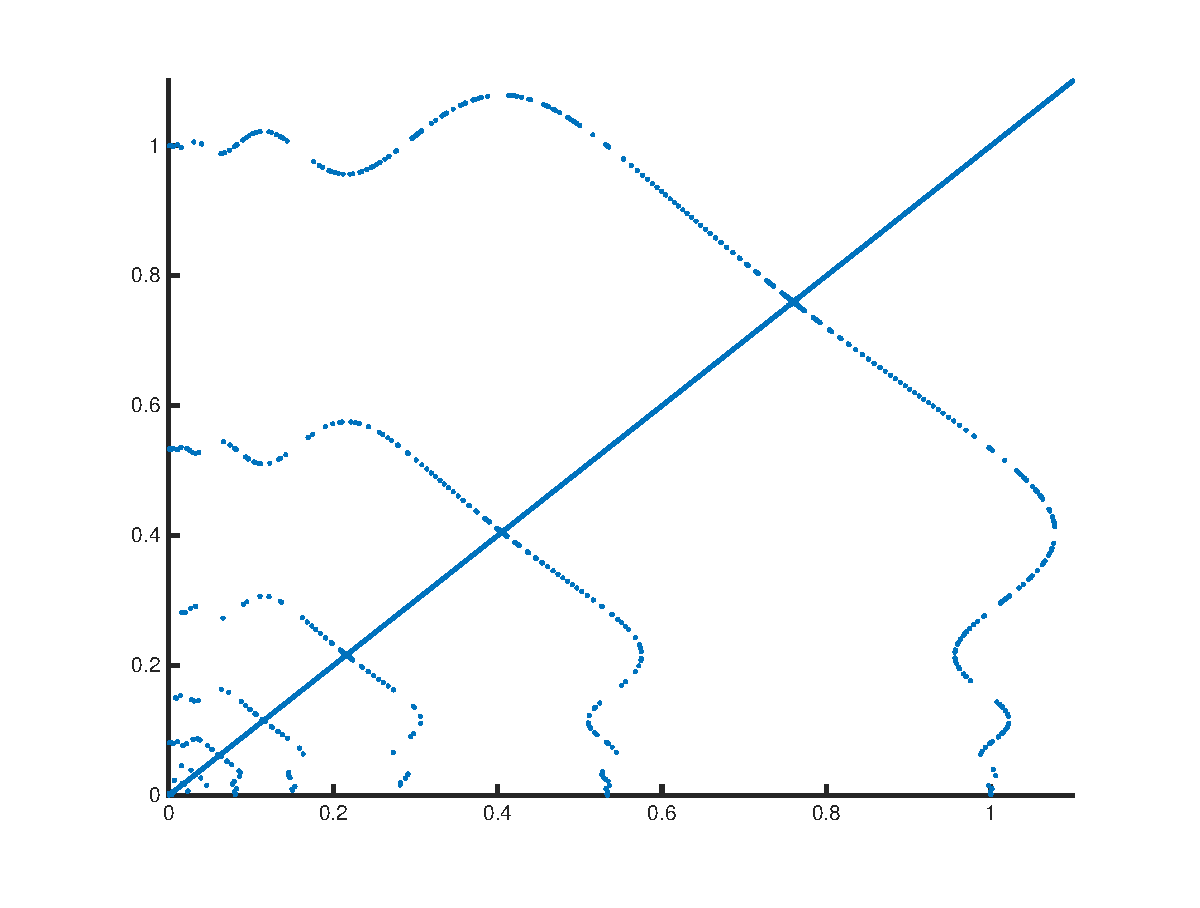
\includegraphics[width=10cm]{zeroset5.eps}
\caption{Zero set of $F(a_0, a_1)$ for $\rho = 5$.}
\end{figure}

We will now prove that such pitchfork bifurcations actually take place.

% Lemma : pitchfork bifurcation

\begin{lemma}\label{pitchfork}
A countable family of pitchfork bifurcations in the zero set of \eqref{defF} occurs along the diagonal at 

\begin{align*}
(a_0, a_1) &= (b_n^*, b_n^*) && n \in \Z
\end{align*}

where 

\begin{equation}
b^*_n = \exp\left(\frac{n \pi}{\rho} \right) \exp \left( -\frac{1}{\rho} \arctan \rho \right)
\end{equation}

Locally, the arms of the pitchfork bifurcations open upwards along the diagonal.

\begin{proof}
First, we need to determine the locations of the hypothesized pitchfork bifurcations along the diagonal. A necessary condition for these to occur is that the first derivative vanishes. Taking the derivative of $F$ with respect to $a_0$ and evaluating it on the diagonal, we have

\begin{align*}
F_{a_0}(a_0, a_0) &= 
\sin \left( - \rho \log a_0 \right)
+ a_0 \cos \left( - \rho \log a_0 \right)- \rho \frac{1}{a_0} \\
&= \sin \left( - \rho \log a_0 \right) - \rho \cos \left( - \rho \log a_0 \right)
\end{align*}

This derivative is 0 if and only if

\begin{align*}
\tan \left( -\rho \log a_0 \right) &=  \rho \\
-\rho \log a_0 &= \arctan \left( \rho\right) - n \pi && n \in \Z \\ 
a_0 &= \exp \left( -\frac{1}{\rho} \arctan \rho + \frac{n \pi}{\rho} \right) && n \in \Z
\end{align*}

Let 

\begin{equation}
b^* = \exp \left( -\frac{1}{\rho} \arctan \rho \right)
\end{equation}

and for $n \in \Z$ let 

\begin{equation}
b^*_n = \exp \left( -\frac{1}{\rho} \arctan \rho + \frac{n \pi}{\rho} \right) 
= \exp\left(\frac{n \pi}{\rho} \right) b^*
\end{equation}

By symmetry, we also have $F_{a_1}(b^*_n, b^*_n) = 0$. Thus the only possible pitchfork bifurcation points are $(a_0, a_1) = (b^*_n, b^*_n)$.\\

At this point, we will verify the rest of the criteria for the pitchfork bifurcation and obtain a leading order approximation for the bifurcation curve. To do this, we will change coordinates so that we can put the equation for $F$ into the normal form of a pitchfork bifurcation. Let 

\begin{align*}
x &= \frac{1}{2}(a_1 - a_0) \\
y &= \frac{1}{2}(a_1 + a_0)
\end{align*}

Inverting this, we have

\begin{align*}
a_0 &= y - x \\
a_1 &= y + x
\end{align*}

Substituting this into the equation for $F(a_0, a_1)$ yields

\begin{equation}\label{Fxy}
F(x, y) = 
(y - x) \sin \left( -\rho \log(y - x) \right) - (y + x) \sin \left( - \rho \log (y + x) \right)
\end{equation}

It is easy to see from \eqref{Fxy} that $F(-x, y) = -F(x, y)$, thus $y$ will be the bifurcation parameter. From the above anod our change of variables, we expect the bifurcations to occur at $(x_0, y_0) = \left(0, b^*_n \right)$.\\

At this point, we need to evaluate a bunch of derivatives at $(x_0, y_0)$. For the first derivatives, we have

\begin{align*}
F_x(x, y) &= -\sin \left( - \rho \log(y - x) \right) - 
\sin \left( - \rho \log(y + x) \right)
+\rho \cos \left( - \rho \log(y - x) \right) + \rho \cos \left( - \rho \log(y + x) \right) \\
F_y(x, y) &= \sin \left( - \rho \log(y - x) \right) - 
\sin \left( - \rho \log(y + x) \right)
-\rho \cos \left( - \rho \log(y - x) \right) + \rho \cos \left( - \rho \log(y + x) \right)
\end{align*}

Plugging in $(x_0, y_0) = \left(0, b^*_n \right)$ and noting that $\sin(\arctan \rho) = \rho / \sqrt{1 + \rho^2}$ and $\cos(\arctan \rho) = 1 / \sqrt{1 + \rho^2}$, it is easy to see that both $F_x(x_0, y_0) = 0$ and $F_y(x_0, y_0) = 0$. \\

For $F_{xx}$, we have

\begin{align*}
F_{xx}(x, y) &= 
-(y-x) \left(-\frac{\rho^2 \sin \left(\rho \log (y-x)\right)}{(y-x)^2}-\frac{\rho
   \cos \left(\rho \log (y-x) \right)}{(y-x)^2}\right)\\
   &+(x+y) \left(-\frac{\rho^2
   \sin \left(\rho \log (x+y)\right)}{(x+y)^2}-\frac{\rho \cos \left( \rho
   \log (x+y)\right)}{(x+y)^2}\right)\\
   &-\frac{2 \rho \cos \left(\rho \log
   (y-x) \right)}{(y-x)}+\frac{2 \rho \cos \left( \rho \log (x+y) \right)}{
   (x+y)}
\end{align*}

A tedious calculation, which can be verified by Mathematica,  tells us that $F_{xx}(x_0, y_0) = 0$. By symmetry, we also have $F_{yy}(x_0, y_0) = 0$, although that it not strictly necessary for the pitchfork. The mixed derivative $f_{xy}$ is

\begin{align*}
F_{xy}(x, y) &= -\frac{\rho^2 \sin \left(\rho \log (y-x)\right)}{(y-x)}-\frac{\rho^2 \sin
   \left(\rho \log (x+y)\right)}{(x+y)}+\frac{\rho \cos \left(\rho \log (y-x)\right)}{(y-x)}+\frac{\rho \cos \left( \rho \log (x+y) \right)}{(x+y)}
\end{align*}

Evaluating this at $(x_0, y_0) = \left(0, b^*_n \right)$ gives us

\begin{align*}
F_{xy}(0, b^*_n) &= \frac{2 \rho}{b_n^*}\left( -\rho \sin \left(\rho \log b_n^*\right) + \cos \left(\rho \log b_n^*\right) \right)\\
&= \frac{2 \rho}{b_n^*}\left( -\rho \sin \left(\rho \log b^* + n \pi \right) + \cos \left(\rho \log b^* + n \pi \right) \right) \\
&= \frac{2 \rho}{b_n^*} (-1)^n \left( \rho \sin \left(\arctan \rho \right) + \cos \left(\arctan \rho \right) \right)\\ 
&= \frac{2 \rho}{b_n^*} (-1)^n \frac{\rho^2 + 1}{\sqrt{1 + \rho^2}} \\
&= (-1)^n 2 \rho \sqrt{1 + \rho^2} \: \exp{\left(\frac{1}{\rho} (\arctan \rho - n \pi) \right)}
\end{align*}

Since $\rho > 0$, this is nonzero. Let $k_1^n = F_{xy}(0, b^*_n)$. \\

Finally, we check the third derivative with respect to $x$. This is another tedious calculation, but after substituting $(x_0, y_0) = \left(0, b^*_n \right)$ we obtain

\begin{align*}
F_{xxx}(0, b_n^*)
&= -(-1)^n 2 \rho \sqrt{1 + \rho^2} \: \exp{\left(\frac{2}{\rho} (\arctan \rho - n \pi) \right)}
\end{align*}

Since $\rho > 0$, this is also nonzero. Let $k_2^n = -F_{xxx}(0, b^*_n)$. \\

We have verified that a pitchfork bifurcation occurs at $(0, b^*_n)$ for $n \in \Z$. Near the bifurcation points $(0, b_n^*)$, we have the following Taylor expansions

\begin{align*}
F(x, y) &= k_1^n x (y - b_n^*) - \frac{k_2^n}{6} x^3 + \text{h.o.t.} \\
&= k_1^n x \left( (y - b_n^*) - \frac{k_2^n}{6 k_1^n } x^2 \right) + \text{h.o.t.} \\
&= k_1^n x \left( (y - b_n^*) - \frac{k_3^n}{6} x^2 \right) + \text{h.o.t.} \\
\end{align*}

where

\begin{equation*}
k_3^n = \exp{\left(\frac{1}{\rho} (\arctan \rho - n \pi) \right)} > 0
\end{equation*}

To leading order, the arms of the pitchforks are upwards-opening parabolas of the form 

\begin{align*}
y &= b_n^* + \frac{k_3^n}{6} x^2
\end{align*}

Since the above change of coordinates is linear, we have shown that pitchfork bifurcations occur in the original coordinate system at $(a_0, a_1) = (b_n^*, b_n^*)$. Since the change of coordinates is a rotation by $\pi/4$, in the original coordinate system, the arms of the pitchforks are, to leading order, parabolas which open upwards along the diagonal.

\end{proof}
\end{lemma}

A plot of the pitchfork parabola in the $(x,y)$ coordinate system is shown below.

\begin{figure}[H]
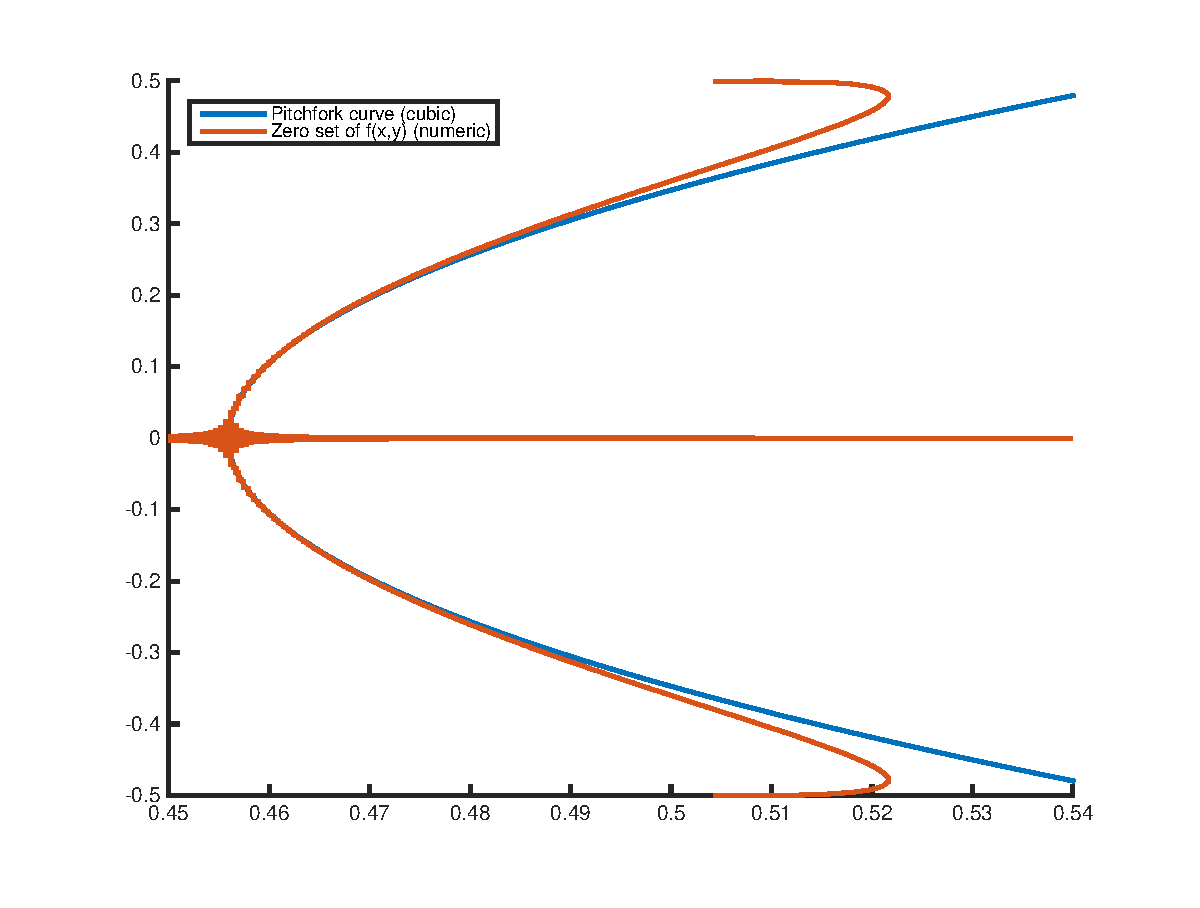
\includegraphics[width=10cm]{pitchfork.eps}
\caption{Pitchfork bifurcation at $(x_0, y_0) = (0, b^*)$ for $\rho = 1$. In this plot, the paramater $y$ is on the horizontal axis.}
\end{figure}

At this point, we only have local information about the zero set of $F(a_0, a_1)$ near the pitchfork bifurcation points. Next, we show that the arms of the pitchfork connect to points on the axes, i.e. that the zero set resembles Figure \ref{fig:Fzeronumeric}. To do this, we construct the following Hamiltonian system

\begin{align}
\dot a_0 &= -F_{a_1}(a_0, a_1) = \sin(-\rho \log a_1) 
- \rho \cos( -\rho \log a_1 )) \\
\dot a_1 &= F_{a_0}(a_0, a_1) = \sin(-\rho \log a_0) 
-\rho \cos( -\rho \log a_0 )
\end{align}

By construction, $F(a_0, a_1)$ is constant along trajectories of this system, and so we can consider $F$ to be an energy function. From Lemma \ref{pitchfork}, we have

\begin{align*}
F_{a_0}(a_0, a_1) &= 0 \iff a_0 = b^*_n, n \in \Z \\
F_{a_1}(a_0, a_1) &= 0 \iff a_1 = b^*_n, n \in \Z
\end{align*}

Thus we have families of nullclines

\begin{align*}
\dot a_0 = 0 &\text{ on } (a_0, b^*_n), n \in \Z \\
\dot a_1 = 0 &\text{ on } (b^*_n, a_1), n \in \Z
\end{align*}

We can now prove the following lemma. Recall that by symmetry we only need to consider the case $a_1 \leq a_0$, i.e. we only need to look at the lower arm of the pitchfork.

% lemma : continuation of pitchfork arms

\begin{lemma}\label{pitchcont}
For the zero set $F(a_0, a_1)$ = 0, the lower arm of the pitchfork at $(b_n^*, b_n^*)$ is a smooth curve with the following properties:

\begin{enumerate}
\item $a_1$ is strictly decreasing along the curve.
\item $a_0 \in (b_n^*, b_{n+1}^*)$ along the curve.
\item The curve terminates at the point $(e^{n \pi/\rho}, 0)$.
\end{enumerate}

The lower arm of the pitchfork can be written as the graph $(x_n^*(a_1), a_1)$ for $a_1 \in [0, b_n^*]$, where $x_n(0) = e^{n \pi/\rho}$ and $x_n(b_n^*) = b_n^*$, and the function $x_n^*$ is smooth.

\begin{proof}

We will look at the lower arm of the pitchfork bifurcation at $(a_0, a_1) = (b_n^*, b_n^*)$. From Lemma \ref{pitchfork}, we know what this looks like locally. To be precise, we can find a point $(a_0^*, a_1^*)$ near $(b_n^*, b_n^*)$ with $b_n^* < a_0^* < b_{n-1}^* $ and $0 < a_1^* < b_n^*$ and a smooth curve connecting them so that $F(a_0, a_1) = 0$ along this cure. From the normal form in Lemma \ref{pitchfork}, this curve must lie below and to the right of the bifurcation point $(b_n^*, b_n^*)$. We note in particular that $F(a_0^*, a_1^*) = 0$. We will show in a series of steps that we can continue this curve uniquely until it meets the $a_0$ axis at $(e^{n \pi/\rho}, 0)$.

\begin{enumerate}

\item First, we show that $e^{n \pi/\rho} \in (b^*_n, b^*_{n+1})$.\\

Recall that

\begin{equation*}
b^*_n = \exp\left(\frac{n \pi}{\rho} \right) \exp \left( -\frac{1}{\rho} \arctan \rho \right)
\end{equation*}

Since $\rho > 0$, $b^*_n < e^{n \pi/\rho}$. We also have 

\begin{equation*}
b^*_{n+1} = \exp\left(\frac{\pi}{\rho} \right) b^*_n = \exp\left(\frac{n \pi}{\rho} \right) \exp \left( \frac{1}{\rho}(\pi - \arctan \rho)\right)
\end{equation*}

Since $\arctan \rho \in (-\pi/2, \pi/2)$, $e^{n \pi/\rho} < b^*_{n+1}$.

\item Next, we show that $\dot a_1 \neq 0$ on the open interval 
$a_0 \in (b^*_n, b^*_{n+1})$.\\

The endpoints the interval lie along the nullclines for $\dot a_1$, thus $\dot a_1 = 0$ at the two endpoints of the interval. There are no other zeros of $\dot a_1 = 0$ between the two endpoints. Consider the point $e^{(2n+1)\pi/(2\rho) }b^*$ which lies inside $(b^*_n, b^*_{n+1})$. At this point,

\begin{align*}
\dot a_1 &= f_{a_0}(e^{(2n+1) \pi / (2\rho)}b^*, a_1) \\
&= \sin(-\rho \log e^{(2n+1) \pi / (2\rho)} b^* ) - \rho \cos( -\rho \log e^{(2n+1) \pi / (2\rho)} b^* ) \\
&= \sin\left(-\rho \left( \frac{(2n + 1)\pi}{2\rho} - \frac{1}{\rho} \arctan \rho \right) \right) - \rho \cos\left(-\rho \left( \frac{(2n + 1)\pi}{2\rho} - \frac{1}{\rho} \arctan \rho \right) \right) \\
&= \sin\left(\arctan \rho - \frac{\pi}{2} - n \pi \right) - \rho \cos\left(\arctan \rho - \frac{\pi}{2} - n \pi \right) \\
&= -\cos\left(\arctan \rho \right) - \rho \sin\left(\arctan \rho\right) \\
&= -(-1)^n \left( \frac{1}{\sqrt{1+\rho^2}} + \rho \frac{\rho}{\sqrt{1+\rho^2}}  \right) \\
&= (-1)^{n+1}\sqrt{1 + \rho^2} \neq 0
\end{align*}

Since $\dot a_1 = f_{a_0}(a_0, a_1)$ is continuous on $[b^*_n, b^*_{n+1}]$, is zero only at the endpoints, and is either negative ($n$ even) or positive ($n$ odd) at a point in between, we conclude that on the open interval $(b^*_n, b^*_{n+1})$, $\dot a_1 < 0$ for $n$ even and $\dot a_1 > 0$ for $n$ odd.

\item Next, we show that the energy $F(a_0, a_1)$ is nonzero on the interior of the line segment joining $(b^*_n, 0)$ to $(b^*_n, b^*_n)$. (The energy is 0 at the endpoints).\\

In the interior of the line segment, the energy is given by

\begin{align*}
F(b^*_n, a_1) &= b^*_n \sin(-\rho \log b^*_n) - a_1 \sin(-\rho \log a_1) && a_1 \in (0, b^*_n)\\
\end{align*}

Let $g(x) = x \sin(-\rho \log x)$, so that $F(b^*_n, a_1) = g(b^*_n) - g(a_1)$. Let $y = -\rho \log x$, so that $x = e^{-y/\rho}$. Then for $x = b^*_n$, $y = -\rho \log b^*_n = \arctan \rho - n \pi$. Making this change of variables, we have $g(y) = e^{-y/\rho} \sin y$. Thus it suffices to show for all $n \in \Z$ that

\begin{align*}
g(\arctan \rho - n \pi) - g(y) &\neq 0 && y \in (\arctan \rho - n \pi, \infty) 
\end{align*}

Taking the derivative of $g$ with respect to $y$, we have

\begin{align*}
g'(y) &= e^{-y/\rho}\left( \cos y - \frac{1}{\rho} \sin y \right)
\end{align*}

In particular, $g'(\arctan \rho - n \pi) = 0$, so $\arctan \rho + n \pi$ is a critical point of $g$. To show it is a local extremum, we evaluate the second derivative.

\begin{align*}
g''(y) &= \frac{e^{-y/\rho}}{\rho^2} \left( \sin y - 2 \rho \cos y - \rho^2 \sin y \right)
\end{align*}

At $y = \arctan \rho - n \pi$, this is

\begin{align*}
g''(y) &= (-1)^n e^{-n \pi /\rho} \frac{e^{-(1/\rho)\arctan \rho}}{\rho^2 \sqrt{1+\rho^2}} \left( \rho - 2\rho - \rho^3 \right) \\
&= (-1)^{n+1} e^{-n \pi /\rho} \frac{e^{-(1/\rho)\arctan \rho}}{\rho^2 \sqrt{1+\rho^2}} \rho \left( 1 + \rho^2 \right) \\
&= (-1)^{n+1} \frac{ \sqrt{1 + \rho^2}}{\rho} e^{-n \pi /\rho} e^{-(1/\rho)\arctan \rho}
\end{align*}

Since $\rho > 0$, $\arctan \rho - n \pi$ is a local maximum for $n$ even and a local minimum for $n$ odd. For $n$ even, since $\arctan \rho - n \pi$ is a local maximum of $g(y) = e^{-y/\rho} \sin y$, and we know exactly how that function behaves, $g(y) < g(\arctan \rho - n \pi)$ whenever $y > \arctan \rho - n \pi$, thus $g(\arctan \rho - n \pi) - g(y) > 0$ for $y \in (\arctan \rho - n \pi, \infty)$. Similarly, if $n$ is odd, $g(\arctan \rho - n \pi) - g(y) < 0$ for $y \in (\arctan \rho - n \pi, \infty)$. In either case, $g(\arctan \rho - n \pi) - g(y) \neq 0$ for all $y \in (\arctan \rho - n \pi, \infty)$.

\item Next, we show that trajectories starting on the lower branch of the pitchfork are confined to a box.\\ 

Consider the box $B$ with corners $(b^*_n, b^*_n)$, $(b^*_{n+1}, b^*_n)$, $(b^*_n, 0)$, and $(b^*_{n+1}, 0)$. The upper left corner is the pitchfork bifurcation point. The initial condition $(a_0^*, a_1^*)$ from which we will continue our solution lies within this box.\\

Within the box, we showed in part 2 that all solutions either move down (for $n$ even) or up (for $n$ odd). If a solution hits the bottom edge of the box, it will stop since the RHS of the ODE is singular there. (Alternatively, the solution will become complex at that point, in which case we are no longer interested in it.)\\

All that remains is to show that the solution starting at $(a_0^*, a_1^*)$ cannot exit the sides. Recall that $F(a_0^*, a_1^*) = 0$ and that solutions are level sets of the energy. Thus $F$ must be 0 along the solution. We showed in part 3 that the sides of the box have nonzero energy. Thus the solution cannot cross the sides of the box.

\item Combining the results above, for $n$ even, a solution starting at $(a_0^*, a_1^*)$ is confined to the box $B$ for $t > 0$. Within the box, we always have $\dot a_1 < 0$. Thus the solution starting at $(a_0^*, a_1^*)$ is strictly decreasing (as $t$ increases) until it hits the $a_0$ axis. The only point on the lower edge of the box which has zero energy is $(e^{n \pi/\rho}, 0)$, and by part 1, this point lies in the interior of the lower edge. Thus the trajectory must terminate at this point. The same result holds for $n$ odd if we take $t < 0$ and consider decreasing $t$.

\item Since $a_1$ is strictly decreasing along the lower arm of the pitchfork, it can be written as the graph $(x_n^*(a_1), a_1)$ for $a_1 \in [0, b_n^*]$, where $x_n(0) = e^{n \pi/\rho}$ and $x_n(b_n^*) = b_n^*$.

\end{enumerate}

\end{proof}
\end{lemma}

Before we continue, we need to address two ``nonuniqueness'' issues in how we have set up the problem.\\

First, if we have constructed a 2-pulse with lengths $(X_0, X_1)$, $X_0 \neq X_1$, it is clear from symmetry of Lin's method that we can also construct a 2-pulse with lengths $(X_1, X_0)$. But since we are on a periodic domain, we can place the origin anywhere we want, thus we see that these two 2-pulses are identical. Thus WLOG we can always take $X_0 \leq X_1$, i.e. $a_0 \geq a_1$.\\

Second, recall that in terms of $r_m$ and $a_i$, the length $X_i$ is given by 

\begin{align*}
X_i &= -(1/ 2 \alpha)\log a_i r_m - \frac{\phi}{2 \beta} 
\end{align*}

If we have constructed a solution using $(a_0, a_1, r_m)$, then must also be able to construct the same solution using $(e^{n/\rho} a_0, e^{n/\rho} a_1, r_{m+n}$ for any $n \in \N$, since those parameters give us the same lengths $(X_1, X_2)$. One way to get uniqueness is to impose an additional condition on which $a_i$ are allowable, as is done in SanStrut. For the 2-pulse, we will impose the following initial condition: $a_0$ must live on the branch of the bifurcation diagram corresponding to the pitchfork bifurcation point $b^*$. \\

Since we have completely characterized the zero set of $F(a_0, a_1)$, we can actually use what we have right now, together with the IFT, to complete the construction of the 2-pulse. If we did that, however, we would lose any information about the bifurcation structure, which will not generically persist once $r_m > 0$. We need to show that for small $r_m$, the bifurcation structure of $G(a_0, a_1, r_m)$ is the same as for $F(a_0, a_1)$. The first thing we will show is that $\tilde{G}$ has the same symmetries as $F$.

% lemma : symmetries of G

\begin{lemma}\label{Gsymm}

As in Lemma \ref{Gchangevar}, for $i = 0, 1$ define

\begin{equation}\label{Gdef}
G_i(a_0, a_1, r_m) = a_i \sin \left( -\rho \log a_i \right) - a_{i-1} \sin \left( -\rho \log a_{i-1} r_m \right) + \mathcal{O}(r_m^{\gamma / 2 \alpha}) = 0 \\
\end{equation}

Then for sufficiently small $r_m$, 

\begin{equation}
G_i(a_0, a_1, r_m) = -G_i(a_1, a_0, r_m)
\end{equation}

\begin{proof}

First, we note that the expression for $G_i$ was obtained by a change of varibles from the equation

\begin{align}
\langle \Psi(0), V_i^+(0) - V_i^-(0) \rangle = 
\langle \Psi(X_i), Q(-X_i) \rangle - \langle \Psi(-X_{i-1}), Q(X_{i-1}) \rangle + R_i
\end{align}

for $i = 0, 1$. This was obtained via Lin's method and is the jump $\xi_i$ between the $i^\pm$ pieces in the direction of $\Psi(0)$. In other words, changing variables back to the $X_i$,

\begin{align}\label{GXi}
G_i(X_0, X_1) = \langle \Psi(0), V_i^+(0) - V_i^-(0) \rangle = \langle \Psi(0), U_i^+(0) - U_i^-(0) \rangle
\end{align}

where the second equality holds since

\begin{align*}
U_i^\pm(x) &= Q^\pm(0, \beta_i^\pm)(x) + V_i^pm(x) 
\end{align*}

and $Q^\pm(0, \beta_i^\pm)(0)$ has no component in $\Psi(0)$. In particular,

\begin{align*}
G_0(X_0, X_1) &= \langle \Psi(0), U_0^+(0) - U_0^-(0) \rangle \\
G_1(X_0, X_1) &= \langle \Psi(0), U_1^+(0) - U_1^-(0) \rangle 
\end{align*}

First, we show that, $G(X_0, X_1)$ as defined in \eqref{GXi} is a well-defined function of the $X_i$, i.e. it has a unique value. Recall that in the first three steps of Lin's method, we solved, in turn, the equations

\begin{align*}
(U_i^\pm)' - F(U_i^\pm) &= 0 \\
U_i^+(X_i) - U_{i+1}^-(-X_i) &= 0 \\
P_{Y^\pm}(U_i^+(0) - U_i^-(0)) &= 0
\end{align*}

where $U_i^\pm(x)$ are functions defined piecewise on a series of intervals determined by the ordered pair $(X_0, X_1)$ and arranged in the standard order, as described above. For sufficiently large $X_i$, each of the three steps yields a unique solution. Thus for a given pair of lengths $(X_0, X_1)$ which are sufficiently large, there is a unique set of functions $U_i^\pm$ in the appropriate function space which satisfies the three equations. Thus \eqref{GXi} is well-defined.
\\

Suppose for an ordered pair of lengths $(X_0, X_1)$ we have a solution $\{ U_0^-(x), U_0^(x), U_1^-(x), U_1^+(x) \}$, pieced together from L to R. Then if swap the $X_0$ and $X_1$ to get the ordered pair $(X_1, X_0)$, the three equations are satisfied by the set of functions $\{ U_1^-(x), U_1^+(x), U_0^-(x), U_0^+(x)\}$, pieced together from L to R. From this, we see that

\begin{align*}
G_0(X_1, X_0) &= \langle \Psi(0), U_1^+(0) - U_1^-(0) \rangle = G_1(X_0, X_1) \\
G_1(X_1, X_0) &= \langle \Psi(0), U_0^+(0) - U_0^-(0) \rangle = G_0(X_0, X_1)
\end{align*}

Next, we note that if we replace $x$ with $-x$, then for the same ordered pair $(X_0, X_1)$, the set of functions $\{ U_1^+(-x), U_1^-(-x), U_0^+(-x), U_0^-(-x)\}$, pieced together from L to R, also satisfies the three equations. By uniqueness, this implies that $U_1^+(0) = U_0^-(0)$ and $U_1^-(0) = U_0^+(0)$. Thus we have

\begin{align*}
G_0(X_0, X_1) &= \langle \Psi(0), U_0^+(0) - U_0^-(0) \rangle \\
&= \langle \Psi(0), U_1^-(0) - U_1^+(0) \rangle \\
&= -\langle \Psi(0), U_1^+(0) - U_1^-(0) \rangle \\
&= -G_1(X_0, X_1) \\
&= -G_0(X_1, X_0)
\end{align*}

Similarly, $G_1(X_0, X_1) = -G_1(X_1, X_0)$. Changing variables back to $(a_0, a_1, r_m)$ yields the result. The condition that the $X_i$ are sufficiently large is equivalent to $r_m$ being sufficiently small.

\end{proof}
\end{lemma}

Next, we show that the pitchfork bifurcation persists for sufficiently small $r_m$. Since we have a Hamiltonian system and thus only have to solve one of the two $G_i$ equations, for convenience we will take $G = G_0$.

% Persistence of pitchfork

\begin{lemma}\label{pitchpersist}

For all $n \in \Z$ there exists $r > 0$ and a unique smooth function $c_n^*: \mathcal{R} \cap [0, r] \rightarrow \R^+$ such that $G(a_0, a_1, r_m)$ has a nondegenerate pitchfork bifurcation at $(c_n^*(r_m),c_n^*(r_m)$. Furthermore, $c_n^*$ is smooth, and

\begin{equation*}
c^*(n, r_m) \rightarrow b^*_n \text{ as } r_m \rightarrow 0
\end{equation*}

\begin{proof}
We make the following assumption: for all derivatives of $G$ with respect to the $a_i$, the remainder term is $\mathcal{O}(r_m^{\gamma / 2 \alpha})$ (or similar). Lemma 6.2 in San98 and Proposition 3.8 in SanStrut have this result up to first derivatives with respect to the $a_i$. I imagine this follows from San93.\\

For simplicity, take $n = 0$, so that we are looking for the persistence of the pitchfork bifurcation at $(b^*, b^*)$. Recall that in Lemma \ref{pitchfork}, we showed that a pitchfork bifurcation occurs at $(b^*, b^*)$ for the equation

\begin{equation}
F(a_0, a_1) = G(a_0, a_1, 0) = a_0 \sin \left( -\rho \log a_0 \right) - a_1 \sin \left( -\rho \log a_1 r_m \right)\\
\end{equation} 

First, as in Lemma \ref{pitchfork}, we change coordinates $(a_0, a_1) \mapsto (x, y)$, so that $(0, b^*)$ is a pitchfork bifurcation point of $G(x, y, 0)$. By Lemma \ref{Gsymm}, in this cooordinate system we have the symmetry $G(-x, y, r_m) = -G(x, y, r_m)$. This implies that $G(0, y, r_m) = 0$ for all $y, r_m$. In other words, the line $x = 0$ consists entirely of equilibria, corresponding to the periodic wavetrain.\\

We now prove the existence of pitchfork bifurcations along this line. Since a necessary condition for a pitchfork to occur is $G_x(x, y, r_m) = 0$, we will look at the system

\begin{equation}
H(x,y,r_m) = (G(x,y,r_m), G_x(x,y,r_m)) = 0
\end{equation}

From Lemma \ref{Gchangevar}, the remainder term of $G_x$ and $G_y$ is order $r_m^{\gamma/2 \alpha}$, so it goes to 0 as $r_m \rightarrow 0$. Thus $G_x(x,y,0) = F_x(x,y)$ and $G_y(x,y,0) = F_y(x,y)$. In particular, $G_x(0,b^*,0) = G_y(0, b^*, 0) = 0$, so $D_{x,y}G(0,b^*,0)$ is singular. Thus, as expected, we cannot use the IFT.\\

We will instead do a Liapunov-Schmidt reduction. In Lemma \ref{pitchfork}, we computed that $F_{xy}(0, b^*) = 2 \rho/b^* \sqrt{1+ \rho^2} \neq 0$. Since the remainder term in $G_{xy}$ decays to 0 as $r_m \rightarrow 0$, we have $G_{xy}(0, b^*, 0) = F_{xy}(0, b^*) \neq 0$. Thus we can use the IFT to solve $H_2 = G_x$ for $y$ in terms of $x$ and $r_m$. By the IFT, there exists $r > 0$, an open interval $(-a, a)$, and a unique function $y = y^*(x, r_m)$ with the same smoothness as $G_x$ such that $y^*(0, 0) = b^*$ and $G_x(x, y^*(x, r_m), r_m) = 0$ for $x \in (-a, a)$ and $r_m < r$.\\

Next, we plug this into the equation for $G$ to get

\begin{equation}
G(x, y^*(x, r_m), r_m) = 0
\end{equation}

As noted above, this has a solution for $x = 0$. It remains to check that a pitchfork bifuration occurs at $(0, y^*(0, r_m), r_m)$. First, since $G(x, y, r_m)$ is an odd function in $x$, $G_y(0, y, r_m) = 0$ and $G({xx}(0, y, r_m) = 0$ for all $x, r_m$. So we get $G_y(0, y^*(0, r_m), r_m) = 0$ and $G_{xx}(0, y^*(0, r_m), r_m) = 0$ for free.\\

All that remains is to show that $G_{xy}$ and $G_{xxx}$ are nonzero at $(0, y^*(0, r_m), r_m)$. Recall that $F_{xy}(0, b^*) \neq 0$. Then since $G_{xy}$ and $y^*$ are smooth, and $G_{xy}(0, y^*(0, r_m), r_m) \rightarrow 0 as r_m \rightarrow 0$. Thus, for sufficiently small $r_m$, $G_{xy}(0, y^*(0, r_m), r_m) \neq 0$. Similarly, from Lemma \ref{pitchfork}, we know that $F_{xxx}(0, b^*) \neq 0$. By the same argument, we conclude that $G_{xxx}(0, y^*(0, r_m), r_m) \neq 0$ for sufficiently small $r_m$.\\

Thus, upon changing variables back to $(a_0, a_1)$ and letting $c^* = y^*$, we have shown the pitchfork bifurcation persists for $r_m < r$. The same argument holds for $b^*_n$ for all $n \in Z$. 

\end{proof}
\end{lemma}

% lemma : peristence of trajectory leading to zero on axis

Now we show that the lower arm of the pitchfork which terminates on the $a_0$ axis persists for sufficiently small $r_m$.\\

We make the following definition.

\begin{definition}
For a function $f:\R \rightarrow \R$, and interval 
$I \subset \R$, and $\epsilon > 0$, the $\epsilon$-\emph{tubular neighborhood of }$f$ is the set

\[
\{ (x, y) : y \in I \text{ and }
x \in (f(y) - \epsilon, f(y) + \epsilon) \}
\] 
\end{definition}

% lemma : lower arm of pitchfork persists

\begin{lemma}\label{tubepersists}

For any $n \in \Z$ and for any interval $I = [0, T]$ with $0 < T < b_n^*$ there exists $r > 0$, $a > 0$ and a unique smooth function $h: I \times \mathcal{R} \cap [0, r] \rightarrow \R$ such that for $r_m < r$, $a_1 \in I$ and $(a_0, a_1)$ in an $a$-tubular neighborhood of $x_n^*$, $G(a_0, a_1, r_m) = 0$ if and only if $a_0 = x_n^*(a_1) + h(a_1, r_m)$.

\begin{proof}

For simplicity, we take $n = 0$, and for convenience we let $x^* = x_0^*$. The proof for general $n \in \Z$ is identical. \\

Recall from Lemma \ref{pitchcont} that the lower arm of the pitchfork starting at $(b^*, b^*)$ is given by $(x^*(a_1), a_1)$, for $a_1 \in [0, b^*]$, where $x^*(0) = 1$ and $x^*(b^*) = b^*$. Recall as well that on this path, $G_{a_0}(x^*(a_1), a_1, 0) = F_{a_0}(x^*(a_1), a_1) \neq 0$ except at $a_1 = b^*$.\\

Choose any interval $I = [0, T]$, where $0 < T < b^*$. Then $G_{a_1}(x^*(a_1), a_1, 0) \neq 0$ for $a_1 \in I$.\\

Let 

\begin{equation}
\tilde{G}(a_0, a_1, r_m) = G(a_0 + x^*(a_1), a_1, r_m)
\end{equation}

Then $\tilde{G}(0, a_1, 0) = 0$ for all $a_1 \in I$, and $\tilde{G}_{a_0}(0, a_1, 0) = G_{a_0}(x^*(a_1), a_1, 0) \neq 0$ for $a_1 \in I$.\\

Define $H: \R \times I \times \mathcal{R} \rightarrow \R$ by

\begin{equation}
H(a_0, a_1, r_m) = a_0 - \tilde{G}_{a_1}(0, a_1, 0)^{-1} \tilde{G}(a_0, a_1, r_m)
\end{equation}

We note that for $a_1 \in I$,

\begin{align*}
H(0, a_1, 0) &= 0 \\
H_{a_0}(0, a_1, 0) &= 1 + \tilde{G}_{a_0}(0, a_1, 0)^{-1 }\tilde{G}_{a_0}(0, a_1, 0) = 0
\end{align*}

Choose any $\theta$ with $0 < \theta < 1$. Then since $\tilde{G}_{a_1}$ is continuous, for each $y \in I$ we can find

\begin{enumerate}
\item An open set $U(y) \subset I$ containing y. Note that this is an open set of $I$, not $\R$.
\item An open interval $V(y) = (-a(y), a(y))$, $a(y) > 0$
\item A real number $r(y) > 0$
\end{enumerate} 

such that $|H_{a_0}(a_0, a_1, r_m)| \leq \theta < 1$ for $a_0 \in U(y)$, $a_1 \in V(y)$, and $r_m < r(y)$.\\

The open sets $\{U(y)\}_{y \in I}$ form an open cover of the compact interval $I$, thus we find a finite subcover, i.e. points $y_1, \dots, y_n \in I$ such that $U(y_1) \cup \dots \cup U(y_n)$ covers $I$. Let $r = \min\{ r(y_1), \dots, r(y_n) \}$. Let $a = \min\{ a(r_1, \dots, a(r_n) \}$ and let $V = (-a, a)$.\\

By construction, $|H_{a_0}(a_0, a_1, r_m)| \leq \theta < 1$ for all $a_0 \in V$, $a_1 \in I$, and $r_m < r$. For $x_1, x_2 \in V$, $a_1 \in I$, and $r_m < r$ we have

\begin{align*}
|H(x_2, a_1, r_m) - H(x_1, a_1, r_m)| &\leq
\sup_{x \in V} |H_{a_0}(x, a_1, r_m)||x_2 - x_1| \\
&\leq \theta |x_2 - x_1|
\end{align*}

Thus $H$ is a uniform contraction with respect to $a_0$. Restrict the domain of $H$ to $V \times I \times \{ r_m < r \}$. If necessary, shrink $V$ (by decreasing $a$) so that we have $H: V \times I \times \{ r_m < r\} \rightarrow V$. Then by the uniform contraction mapping principle, for all $a_1 \in I$ and all $r_m < r$, the map $H(\cdot, a_1, r_m)$ has a unique fixed point $h(a_1, r_m)$. The function $h$ is smooth, since $H$ (and $G$) are smooth.\\

From the definition of $H$ and the fact that $\tilde{G}_{a_1}(0, a_1, 0)^{-1} \neq 0$ for all $a_1 \in I$, we see that $a_0$ is a fixed point of $H$ with parameters $a_1$ and $r_m$ if and only if $\tilde{G}(a_0, a_1, r_m) = 0$. Thus, given $a_1 \in I$ and $r_m < r$, $h(a_1, r_m)$ is the unique value of $a_0$ such that $\tilde{G}(a_0, a_1, r_m) = 0$. Since $\tilde{G}(0, a_1, 0) = 0$, by uniqueness $h(a_1, 0) = 0$. For fixed $r_m < r$, the curve $h(a_1, r_m)$ is smooth, and $|h(a_1, r_m)| < a$.\\

Thus there exists $r > 0$ and an open interval $(-a, a)$ such that for any $r_m < r$, $a_1 \in I$, and $|a_0| < a$, $\tilde{G}(a_0, a_1, r_m) = 0$ if and only if $a_0 = h(a_1, r_m)$.\\

Since $\tilde{G}(a_0, a_1, r_m)$ if and only if $G(a_0 + x^*(a_1), a_1, r_m) = 0$, we conclude that for $r_m < r$, $a_1 \in I$ and $(a_0, a_1)$ in an $a$-tubular neighborhood of $x^*$, $G(a_0, a_1, r_m) = 0$ if and only if $a_0 = x^*(a_1) + h(a_1, r_m)$.

\end{proof}
\end{lemma}

For small $r_m$, we shown persistence of the pitchfork bifurcation and the portion of the zero level set of $F$ which meets the $a_0$ axis. The final thing we need to show is to put these pieces together and show that for sufficiently small $r_m$ we have a smooth curve connecting the pitchfork bifurcation point to the $a_0$ axis.

% lemma : persistence of lower arm of pitchfork

\begin{lemma}\label{lowerarmpersists}

For all $n \in \Z$, there exists $r > 0$ such that for $r_m < r$ the zero level set of $G_(a_0, a_1, r_m)$ contains a smooth curve joining $c_n^*(n, r_m)$ to a point on the $a_0$ axis. \\

On this curve, $a_1$ is strictly decreasing from $c^*(n, r_m)$ to 0. Thus for each $n \in \Z$ there is a smooth function $a_0^*(n, a_1, r_m)$ defined for $a_1 \in (0, c^*(n, r_m)$ such that 

\begin{equation}
G(a_0^*(n, a_1, r_m), a_1, r_m) = 0 \text{  for  }
a_1 \in [0, c^*(n, r_m)]
\end{equation}

Furthermore, we have the following limits

\begin{align*}
\lim_{a_1 \rightarrow c_n^*(r_m)} a_0^*(n, a_1, r_m) &= c_n^*(r_m) \\
\lim_{a_1 \rightarrow 0} a_0^*(n, a_1, r_m) &= e^{n \pi / \rho} + h(0, r_m)
\end{align*}

\begin{proof}
As in the previous lemma, we will do this for $n = 0$. The case for $n \in \Z$ is similar.\\

\begin{enumerate}

\item Choose $r > 0$ such that the results of Lemmas 
\ref{pitchpersist} and \ref{tubepersists} apply. 

\item Let $c_0^*(r_m)$ be as defined in Lemma \ref{pitchpersist}, and for convenience let $c^* = c_0^*$.

\item At this point, fix $r_m < r$. Since all pitchfork bifurcations are topologically conjugate, there exists $\epsilon_0 > 0$, $\epsilon_1 > 0$, and a unique diffeomorphism $H_m: B(b^*, \epsilon_0) \rightarrow B(c^*, \epsilon_1)$, all of which depend on $r_m$, such that

\begin{equation}
G(a_0, a_1, 0) = 0 \iff G(H_m(a_0, a_1), r_m) = 0
\end{equation}

We can assume WLOG that the $\epsilon_0, \epsilon_1$ are the largest radii for which this result holds.

\item For this value of $r_m$, using Lemma \ref{tubepersists} with interval $I_0 = [0, b^* - \epsilon_0/2]$, there exists a unique function $h: I_0 \times \mathcal{R} \cap [0, r] \rightarrow \R$ such that

\begin{equation}
G(a_0, a_1, r_m) = 0 \iff a_0 = x^*(a_1) + h(a_1, r_m)
\end{equation}

where $x^* = x_0^*$ is defined in Lemma \ref{pitchcont}. 

\item Let $I_1 = (b^* - \epsilon_0, b^* - \epsilon_0/2)$. Consider the curve $\Gamma_1$ defined by

\begin{align*}
\Gamma_1 = \left\{ (x^*(a_1), a_1) : a_1 \in I_1 \right\}
\end{align*}

Since $\Gamma_1 \subset B(b^*, \epsilon_0)$ and $G(a_0, a_1, 0) = 0$ for $(a_0, a_1) \in \Gamma_1$, $G(H_m(a_0, a_1), r_m) = 0$ for $(a_0, a_1) \in \Gamma_1$. But we also have $G(x^*(a_1) + h(a_1, r_m), a_1, r_m) = 0$, i.e. $G(a_0 + h(a_1, r_m), a_1, r_m) = 0$ for $(a_0, a_1) \in \Gamma_1$. Since the diffeomorphism $G$ is unique, this implies 

\begin{equation}\label{middlejoin}
H_m(a_0, a_1) = (a_0 + h(a_1, r_m), a_1)
\end{equation}

for $(a_0, a_1) \in \Gamma_1$.

\item Let $\Gamma$ be the lower part of the pitchfork at $b^*$ for $r_m = 0$, i.e. 

\begin{equation}
\Gamma = \left\{ (x^*(a_1), a_1) : a_1 \in [0, b^*] \right\}
\end{equation}

Thus we can define the piecewise function $H_1: \Gamma \rightarrow \R^+ \times R^+$ by

\begin{equation}
H_1(a_0, a_1) = \begin{cases}
H(a_0, a_1) & a_1 \in (b^* - 3 \epsilon_0/4, b^*] \\
(a_0 + h(a_1, r_m), a_1) & a_1 \in [0, b^* - 3 \epsilon_0/4]
\end{cases}
\end{equation}

By \eqref{middlejoin}, the two pieces of $H_1$ agree at the join point at $a_1 = b^* - 3 \epsilon_0/4$. Since both pieces are smooth and both pieces agree on the interval $a_1 \in (b^* - \epsilon_0, b^* - \epsilon_0/2)$, $H_1$ is smooth.\\

Let $\Gamma(r_m) = H_1(\Gamma)$. Then $\Gamma$ is a smooth curve connecting $c^*$ to a point on the $a_0$ axis. Since on the two pieces $a_1$ is strictly decreasing, we can write $\Gamma(r_m)$ as a graph over $a_0$.

\end{enumerate}
\end{proof}
\end{lemma}

% put it all together

We collect the results so far in the following proposition.

% proposition : existence in terms of a_i

\begin{proposition}\label{2pera}
Assume Hypothesis \ref{assumptions} and Hypothesis \ref{spechyp}. Then there exists $r > 0$ such that for each $r_m < r$, there exists a 1-paramater family of 2-periodic solutions to \eqref{generaleq}, paramaterized by $a_1 < a_0$. The ``length paramaters'' of the 2-periodic solution are given by

\begin{align}
(a_0, a_1) &= ( a_0^*(0, a_1, r_m), a_1 ) && a_1 \in (0, c_0^*(r_m))
\end{align}

\end{proposition}

We now change variables back to the original lengths $X_i$ and state this result as the following theorem.

% Theorem : in terms of lengths X_i

\begin{theorem}
Assume Hypothesis \ref{assumptions} and Hypothesis \ref{spechyp}. Then there exists $M \in \N_0$ such that for $m \in \N_0 \cap [M, \infty)$ there exists a 1-parameter family of 2-periodic solutions, paramaterized by $X_1 > X_0$. $X_0$ is given by

\begin{equation}\label{X0}
X_0 = \frac{\pi}{2 \beta}m 
- \frac{1}{2 \alpha} \log(\tilde{a}_0(X_1, r_m)) + C
\end{equation}

where $C$ is a constant, and $\tilde{a}_0(X_1, r_m) \rightarrow 1$ as $(X_1, r_m) \rightarrow (\infty, 0)$.

\begin{proof}
This follows from Proposition \ref{2pera} by a change of variables. Using the definitions of $a_i$ and $r_m$from the proof of Lemma \ref{Gchangevar},

\begin{align*}
X_0 &= -\frac{1}{2 \alpha} \log ( a_0^*(0, a_1, r_m) r_m) - \frac{\phi}{2 \beta} \\
&= -\frac{1}{2 \alpha} \log ( a_0^*(0, a_1, r_m))
- \frac{1}{2 \alpha} \log(r_m) - \frac{\phi}{2 \beta} \\
&= -\frac{1}{2 \alpha} \log ( a_0^*(0, a_1, r_m))
- \frac{1}{2 \alpha} \log \left( e^{-(\pi \alpha/\beta)m}\right) - \frac{\phi}{2 \beta} \\
&= \frac{\pi}{2 \beta} m - \frac{1}{2 \alpha} \log( a_0^*(0, a_1, r_m)) + C
\end{align*}

where $C = - \phi/2 \beta$. Since $a_1 = e^{-2\alpha X_1}e^{-\alpha \phi / \beta}\frac{1}{r_m}$, let

\begin{align}
\tilde{a}_0(X_1, r_m) = a_0^*\left(0, e^{-2\alpha X_1}e^{-\alpha \phi / \beta}\frac{1}{r_m}, r_m)\right)
\end{align}

Then 

\begin{align*}
X_0 &= \frac{\pi}{2 \beta} m - \frac{1}{2 \alpha} \log( \tilde{a}_0(X_1, r_m)) + C
\end{align*}

The limits on $\tilde{a}_0$ follow from Lemmas \ref{tubepersists} and \ref{lowerarmpersists}.

\end{proof}
\end{theorem}

% corollary : apply to KdV5

\begin{corollary}
For KdV5, if $c > 0$ there exists a $2$-pulse solution $q_2(x)$. This solution can be written piecewise as in [], and bounds on the pieces are given in that theorem.

\begin{proof}
All we need to do is verify the assumptions in Hypothesis \ref{assumptions} and Hypothesis \ref{spechyp} for KdV5. The assumptions in Hypothesis \ref{assumptions} are discussed in the opening section, except for the transversality condition, which is a standard assumption in the literature. For Hypotehsis \ref{spechyp}, for $c > 0$, the spectrum of $DF(0)$ is given by $\nu = \pm \alpha \pm \beta i$, where $\alpha, \beta > 0$.
\end{proof}

\end{corollary}

\end{document}